\documentclass[12pt,a4paper]{report}

%Allgemeine Dokumenteigenschaften
\usepackage[top=3cm,left=4cm, bottom=3cm, right=2cm]{geometry}
\usepackage[onehalfspacing]{setspace}

%Einstllunge für die Text- und Spracheigenschaften
\usepackage[T1]{fontenc}
\usepackage[utf8x]{inputenc}
\usepackage[ngerman]{babel}
\usepackage{helvet}
\renewcommand{\familydefault}{\sfdefault}

\usepackage{chemfig}
\usepackage{mhchem}


\usepackage{amssymb}
\usepackage{amsmath}
\usepackage{booktabs}

\usepackage{upgreek}
\usepackage{textcomp}


\usepackage{hyperref}
\usepackage{blindtext}

\usepackage[labelfont=bf]{caption}

\usepackage{titlesec}
\titlespacing{\chapter}{0pt}{-25pt}{10pt}
\titleformat{\chapter}{\LARGE\bfseries}{\thechapter\ }{0.1em}{}
\titleformat{\section}{\Large\bfseries}{\thesection\ }{0.1em}{}
\titleformat{\subsection}{\large\bfseries}{\thesubsection\ }{0.1em}{}


\begin{document}

\begin{titlepage}
	\newgeometry{top=2.5cm,left=0.5cm, bottom=2.5cm, right=0.5cm}
	\centering
	{\LARGE \textbf{Lab on a chip}\par}
	\vspace{1cm}
	{\large\MakeUppercase{Vertieferarbeit}\par}
	\vspace{1cm}
	\vspace{0.5cm}
	{im Studiengang Chemie M. Sc.\par}
	\vspace{0.5 cm}
	\vspace{2 cm}
	\makebox[3.6cm][s]{Universität Leipzig} \\
	\makebox[6.6cm][s]{Fakultät für Chemie und Mineralogie} \\
	\vspace{2cm}
	\makebox[6.5cm][s]{eingereicht von Maria Monossova} \\
	\vspace{0.35cm}
	\makebox[6.5cm][s]{Betreuer: Prof. Dr. Bernd Abel} \\
	\vspace{0.35cm}
	\makebox[6.5cm][s]{Zweitgutachter: Dr. Christian Laube} 
	\vfill
	{Leipzig, 17.10.2022   \par}
	
\end{titlepage}
	\chapter{Zusammenfassung}
	\noindent \ce{Zn^{2+}} ist das zweithäufigste Übergangsmetallion im menschlichen Körper und ist an einer Vielzahl biologischer Prozesse beteiligt. Die Entwicklung eines empfindlichen und selektiven Nachweises für \ce{Zn^{2+}}-Ionen ist daher von entscheidender Bedeutung. In dieser Arbeit wurde die Einsatzfähigkeit eines Calix[4]arens als Fluoreszenzsensor für \ce{Zn^{2+}} untersucht, dessen unterer Ring mit einer Schiffschen Base substituiert wurde. Die spektroskopischen Eigenschaften wurden mittels UV/Vis- und Fluoreszenzspektroskopie untersucht. Die Änderung der Fluoreszenz wurde auf einen CHEF-Effekt und die Isomerisierung der C=N Bindung zurückgeführt. Es wurde ein Immobilisierungsansatz und ein Flowversuch verfolgt. 
	\tableofcontents
	\chapter{Einleitung}
	\noindent Metallionen sind an vielzähligen biologischen Prozessen beteiligt und spielen demnach eine zentrale Rolle im medizinischen Sektor. Dabei können sich sowohl ungewöhnlich hohe wie niedrige Ionenkonzentrationen schädlich auf die menschliche Gesundheit auswirken.\\
	\ \\
	So ist beispielsweise Zink ein essentielles Metall, welches überwiegend in den Zellen vorkommt und daher an strukturellen, katalytischen und regulatorischen Aufgaben beteiligt ist. Obwohl Zink nicht giftig ist, kann ein Überschuss die menschliche Gesundheit beeinträchtigen: So wurde ein Ungleichgewicht der Zinkkonzentration mit Brustkrebs, Parkinson, Alzheimer und Diabetes der Typen 1 und 2 in Verbindung gebracht. Ein Zinkmangel kann dagegen zu schweren Stoffwechsel- und Entwicklungsstörungen führen.\\
	\ \\
	Außerhalb des menschlichen Körpers ist die selektive Verfolgung von \ce{Zn^{2+}}-Ionen in den Umwelt- und Biowissenschaften von großer Bedeutung: So führt der industrielle Eintrag von Zink in die Umwelt zu einer erhöhten mikrobiellen Aktivität, welche die Fruchtbarkeit des Bodens beeinträchtigt. \\
	\ \\
	Dabei stellt der Nachweis von \ce{Zn^{2+}}-Ionen aufgrund seiner elektronischen Konfiguration, die spektroskopisch und magnetisch inaktiv ist, eine Herausforderung dar. In dieser Arbeit soll eine mit einer Schiffschen Base versehene Calix[4]areneinheit untersucht werden, welche über ein PET-basierte Änderung seiner Fluoreszenzeigenschaften als Zinksensor fungieren soll.\footnote{A. Waheed, T. Ahmad, M. Haroon, N. Ullah, ChemistrySelect 2020, 5, 5300. }
	\chapter{Theoretischer Teil}
	\section{Chemische Struktur und Fluoreszenz}
	Organische Moleküle besitzen meist eine gerade Elektronenzahl. Dabei befinden sich je zwei Elektronen mit antiparallelem Spin in einem Orbital, sodass sich ein Gesamtspin von S = 0 ergibt. Dem folgt eine Multiplizität  von M = 2S + 1 = 1. Folglich entspricht der elektronische Grundzustand dieser Moleküle einem Singulett. Aus dem Interkombinationsverbot folgt, dass elektronische Übergänge lediglich zwischen Zuständen gleicher Multiplizität erlaubt sind, sodass die Absorptions- und Emissionsspektren organischer Moleküle in der Regel von Übergängen zwischen dem elektronischen Grundzustand \ce{S_0} und höheren Singulettzuständen \ce{S_n} dominiert werden.\\
	\ \\
	Die Anregung von Wellenlängen aus gebundenen $\sigma$-Orbitalen erfordert zumeist Wellenlängen unterhalb von 200 nm, während für die Anregung von $\pi$-Elektronen üblicherweise geringere Energien erforderlich sind, sodass diese im nahen UV und gegebenenfalls sogar im sichtbaren Bereich des Spektrums anzutreffen sind.\footnote{F. Hinderer, UV VIS- und Fluoreszenzspektroskopie, 2020, S. 25-26}\\
	\ \\  
	Die relative Energie der Molekülorbitale ist durch verschiedene Faktoren beeinflussbar. Die deutlichste Wirkung tritt bei der Konjugation von Doppelbindungen auf. Hier gilt, dass sich mit zunehmender Konjugation eine langwellige Verschiebung der Lichtabsorption beobachten lässt, wobei gleichzeitig die Intensität der Absorptionsbanden zunimmt. Dieser Effekt lässt sich auf die zunehmende Annäherung von HOMO und LUMO zurückführen. Neben der Konjugation spielen auch Substituenten am Aromaten eine entscheidende Rolle für den Energiegehalt der Orbitale. Dabei führen ortho- und paradirigierende Substituenten durch die Erhöhung der Elektronendichte des Aromaten im Allgemeinen zu einer Zunahme der Fluoreszenzintensität und einer bathochromen Verschiebung, wohingegen metadirigierende Substituenten die Fluoreszenzintensität aus dem gegenteiligen Grund verringern und eine hypsochrome Verschiebung bewirken. \footnote{S. Schieffer, Intra- und Intermolekularer Elektronentransfer bei 4,5-Dimethoxyphthalimiden und Perylen-3,4,9,10-tetracarboxydiimiden: Fluoreszenz und Photochemie, 2002, S. 6-7}
	\section{PET-basierte Fluoreszenzsensoren}
	\subsection{PET und CHEF}
	Die Detektion eines Analyten mittels eines Chemosensors basiert oftmals auf einer Fluoreszenzänderung, welche sich auf  verschiedene photophysikalische Mechanismen zurückführen lässt. In diesem Abschnitt soll der \textnormal{photoinduzierte Elektronentransfer} (\textbf{PET}) erläutert werden, welcher die Grundlage der nachfolgenden Untersuchungen bildet.\\
	\ \\
	Der PET-Prozess lässt sich anhand der Grenzorbitaltheorie veranschaulichen. Wird ein Fluorophor mit Licht passender Energie bestrahlt, erfolgt die Anregung eines Elektrons vom HOMO zum nächstgelegenen LUMO. Relaxiert das im LUMO befindliche Elektron im Anschluss unter Abgabe eines Photons, kommt es zur Fluoreszenz. Befindet sich jedoch ein freies Elektronenpaar in einem dem Fluorophor benachbarten Orbital und liegt dessen Energie zwischen der seines HOMOs und LUMOs,  wird die Fluoreszenz durch den PET-Prozess unterbunden.\\
	\ \\
	Das Elektronendefizit im HOMO des Fluorophors wird nach der Anregung durch ein Elektron des HOMOs eines Elektronendonors gefüllt. Damit wird die Relaxation des im LUMO befindlichen Elektrons verhindert, wodurch die überschüssige Energie nicht als Fluoreszenz abgegeben werden kann.\\
	\ \\
	Wird das freie Elektronenpaar des Donors an einen Analyten gebunden, wird sein HOMO energetisch abgesenkt und liegt dann unter dem HOMO des Fluorophors. Danach kann die Elektronenübertragung  hier nicht mehr erfolgen, sodass das zuvor angeregte Elektron in seinen Grundzustand relaxieren kann. Damit kann die zuvor durch PET unterdrückte Fluoreszenz detektiert werden (\textbf{\autoref{fig:CHEF}}). Das zugrundeliegende Konzept für die Funktionsweise solcher Chemosensoren basiert meist auf der 
	Komplexierung oder Chelatisierung mit dem Analyten. Folglich wird der Effekt der eintretenden Fluoreszenz infolge einer Komplexierung 
	als \textnormal{ chelation-induced enhanced fluorescence} (\textbf{CHEF}) bezeichnet.\footnote{Harun Taş. Synthese und Analytik von neuartigen
	8-Aminochinolin-basierten Zn-Chemosensoren. S. 7-9}
	\newpage 
	\begin{figure}[h!]
		\centering
		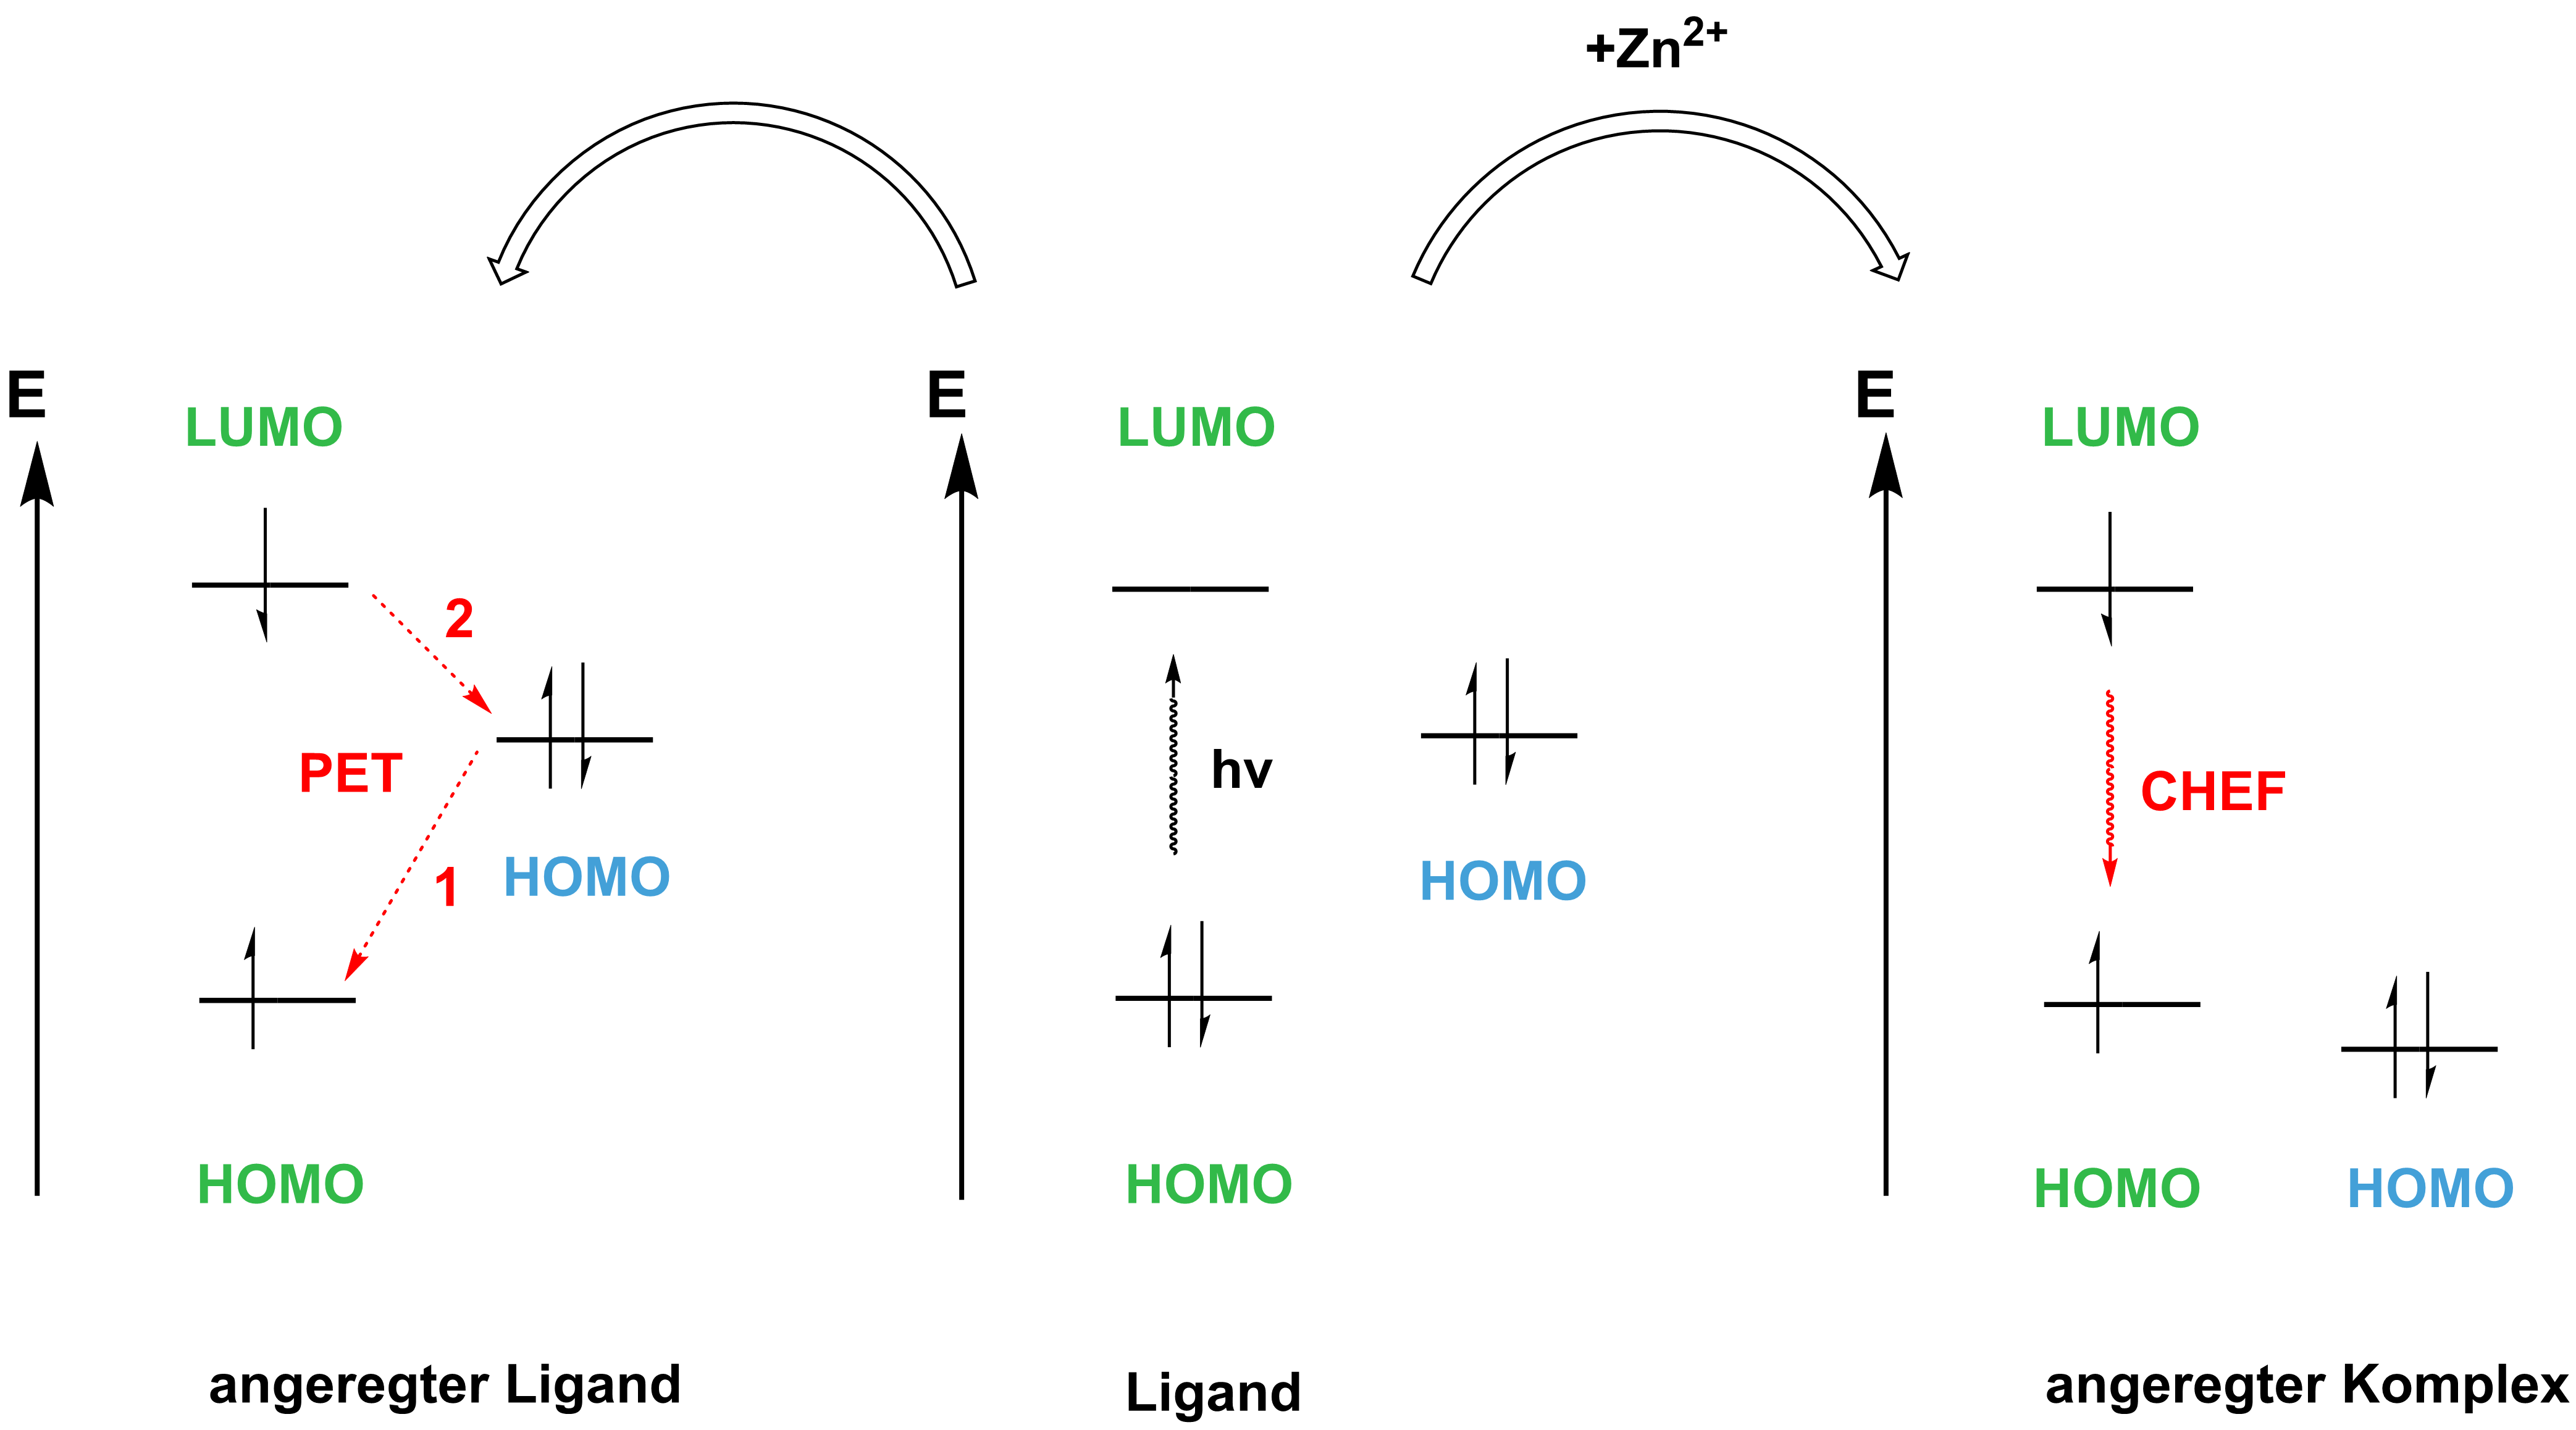
\includegraphics[width=\textwidth]{PETCHEF.png}
		\caption{\textit{Molekülorbitalschema des CHEF-Prozesses: Durch die Zugabe eines Analyten wird das freie Elektronenpaar des Elektronendonors gebunden, sodass sein HOMO energetisch abgesenkt wird. Danach kann das angeregte Elektron des Fluorophors unter Emission von Fluoreszenzstrahlung relaxieren (CHEF).}}
		\label{fig:CHEF}
	\end{figure} 
	\subsection{Aufbau des Fluoreszenzsensors}
	Bei einem PET-basierten Fluoreszenzsensor stehen PET und Fluoreszenz als zwei Hauptwege der Desaktivierung miteinander in Konkurrenz. Durch die Bindung des Analyten wird diese Konkurrenz beeinflusst.\\
	\ \\
	Damit stellen sich folgende Anforderungen an die Struktur des  Chemosensors (\textbf{\autoref{fig:FS}}): Es muss eine \textnormal{fluorophore Gruppe} vorhanden sein, welche als Elektronenakzeptor dient. Typischerweise handelt es sich hierbei um aromatische Systeme. Sie ist über einen aliphatischen \textnormal{Spacer} mit einem \textnormal{Rezeptor} verbunden. Letzterer ist in der Lage den Analyten selektiv und reversibel zu binden und dient außerdem als Elektronendonor. Häufig finden sich in den Rezeptoren elektronenreiche Heteroatome wie z. B. Stickstoffatome, welche imstande sind durch ihre freien Elektronen eine mögliche Fluoreszenz zu quenchen. Innerhalb dieses Systems erfolgt der PET vom Rezeptor auf den Fluorophor. Durch die Bindung des Rezeptors an einen Analyten wird dieser Prozess verhindert oder stark reduziert, wodurch der Chemosensor fluoresziert.\footnote{A. Laubach. Entwicklung fluoreszierender Chemosensoren zur
	Untersuchung von Adenosintriphosphat auf
	Zelloberflächen. S. 9-10}
	\begin{figure}[h!]
		\centering
		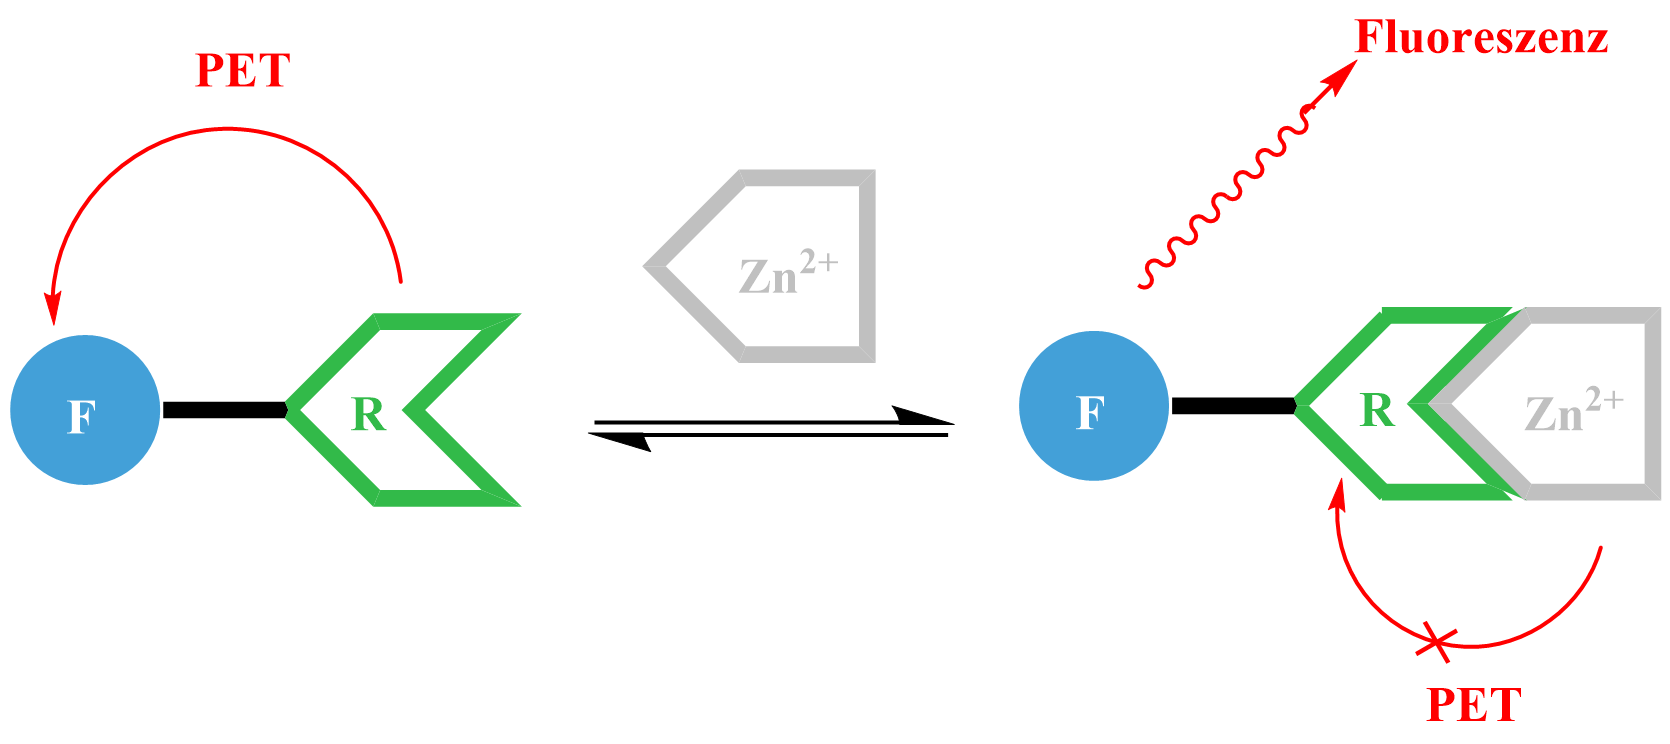
\includegraphics[width=0.8\textwidth]{Sensor.png}
		\caption{\textnormal{\textit{Schema eines PET-basierten Fluoreszenzsensors. Der freie Rezeptor (Elektronendonator) überträgt Elektronen auf den Fluorophor (Elektronenakzeptor). Wird
		der Rezeptor an einen Analyten gebunden, wird PET verhindert, wodurch der Sensor fluoresziert.}}} 
		\label{fig:FS}
	\end{figure}
	\subsection{Calixarene und Schiffsche Basen}
	Calixarene erlangten in den letzten drei Jahrzehnten aufgrund ihrer einzigartigen molekularen Struktur und der vergleichsweise einfachen Funktionalisierung große Bedeutung in der Wirts-Gast-Chemie. In der Struktur der Calixarene existieren zwei Stellen, welche eine Modifikation zulassen, wobei diese unabhängig voneinander behandelt werden können: Zum einen ist die Substitution der phenolischen Hydroxygruppen möglich (unteres Band), zum anderen die Substitution in der para-Position zu den OH-Gruppen (oberes Band), vgl. \textbf{\autoref{fig:Calixarenstruktur}}. Auf diese Weise können verschiedene funktionelle Gruppen eingeführt werden, die in entgegengesetzte Richtungen weisen. Solche modifizierten Calixaren-Derivate haben zusätzliche Bindungsstellen, die die Bindungsfähigkeiten im Vergleich zu den Ausgangs-Calixarenen erhöhen und bieten eine ideale Plattform für die Entwicklung von Rezeptoren für Ionen in Abhängigkeit von der Funktionalisierung.\\
	\ \\ 
	Fluoreszenzsensoren, welche auf der Einbindung von Schiffschen Basen beruhen, erlangten aufgrund ihrer Sensibilität und Sensitivität sowie dem mit der Herstellung verbundenen geringen Kostenaufwand zunehmende Bedeutung. Zwei Effekte führen zu einer geringen Fluoreszenz von Schiffbasenliganden: die Isomerisierung der C=N Bindung sowie der vom freien Elektronenpaar des Stickstoffatoms ausgehenden PET-Effekt. Die Emissionsintensität kann jedoch durch die Unterdrückung der
	C=N-Isomerisierung im angeregten Zustand sowie durch den CHEF-Mechanismus erhöht werden.\footnote{S. Erdemir, S. Malkondu, O. Kocyigit: A reversible calix[4]arene armed phenolphthalein based fluorescent probe for the detection of Zn2+ and an application in living cells, Luminescence, 2018, S. 1}
	\begin{figure}[h!]
		\centering
		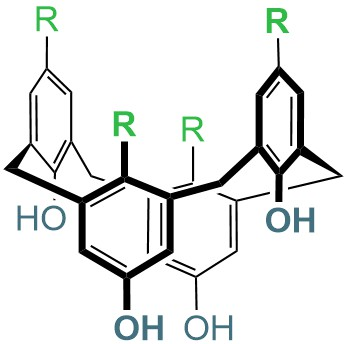
\includegraphics[width=0.3\textwidth]{Calixarenstruktur.png}
		\caption{\textnormal{\textit{Calixarene sind aus Phenoleinheiten aufgebaute Makrocyclen, welche jeweils in ortho-Stellung zur OH-Gruppe über Methylenbrücken verbunden sind}.}} 
		\label{fig:Calixarenstruktur}
	\end{figure}
	\begin{figure}[h!]
		\centering
		\includegraphics[width=0.2\textwidth]{SchiffscheBase.png}
		\caption{\textnormal{\textit{Die Isomerisierung der C=N-Bindung in Schiffbasenliganden führt zu einer Verringerung seiner Fluoreszenz}.}} 
		\label{fig:Schiffsche Base}
	\end{figure}
	\section{Vorteile des Lab on a chip-Systems}
	Lab on a Chip-Systeme können als verkleinerte chemische Verarbeitungsanlagen betrachtet werden. Dabei ermöglichen sie die Miniaturisierung komplexer Analysen, wodurch der Verbrauch der benötigten  Reagenzien drastisch verringert wird. Demnach werden die damit verbundenen Kosten stark reduziert. Ihr Potenzial erstreckt sich auch auf die Möglichkeit der Automatisierung repetitiver Vorgänge, sodass eine Erhöhung des Probendurchsatzes erreicht werden kann. Gleichzeitig steigt die Reproduzierbarkeit der Ergebnisse, wodurch eine insgesamt bessere Datenlage geschaffen wird. Hier spielt insbesondere die Möglichkeit der Integration aufeinanderfolgender Schritte in eine Plattform eine bedeutende Rolle.\\
	\ \\
	Die Lab on a chip-Technologie zählt bereits zum wichtigsten Anwendungsbereich der Mikrofluidik. In den letzten zwei Jahrzehnten hat sie sich zu einem bedeutenden Forschungsgebiet der Biomedizintechnik entwickelt. Hier stellt die Anwendung in der Krankheitsdiagnostik eine vorrangige Rolle.\footnote{A. W. Chow: Lab-on-chip: Opportunities for chemical engineering, AIChE Journal, New York Bd. 48, 2002, S. 1590}
	\chapter{Zielsetzung}
	\noindent Ziel dieser Arbeit ist die Zinkdetektion mittels eines Calix[4]arenliganden, welcher auf einem Lab on a chip-System angewendet wird. Dabei sollen zwei Ansätze: Die \textnormal{Immobiliserung}  (\textbf{\autoref{fig:Immo}}) und ein \textnormal{Flowaufbau} (\textbf{\autoref{fig:Flowansatz}}) verfolgt werden.\\
	\ \\
	Bei der Immobilisierung soll der Ligand mittels Kryogel direkt auf den Chip gedruckt werden. Infolge der Entmischung soll ein Porensystem entstehen, durch welches die Zinklösung hindurchgepumpt werden kann.
	\begin{figure}[h!]
			\centering
			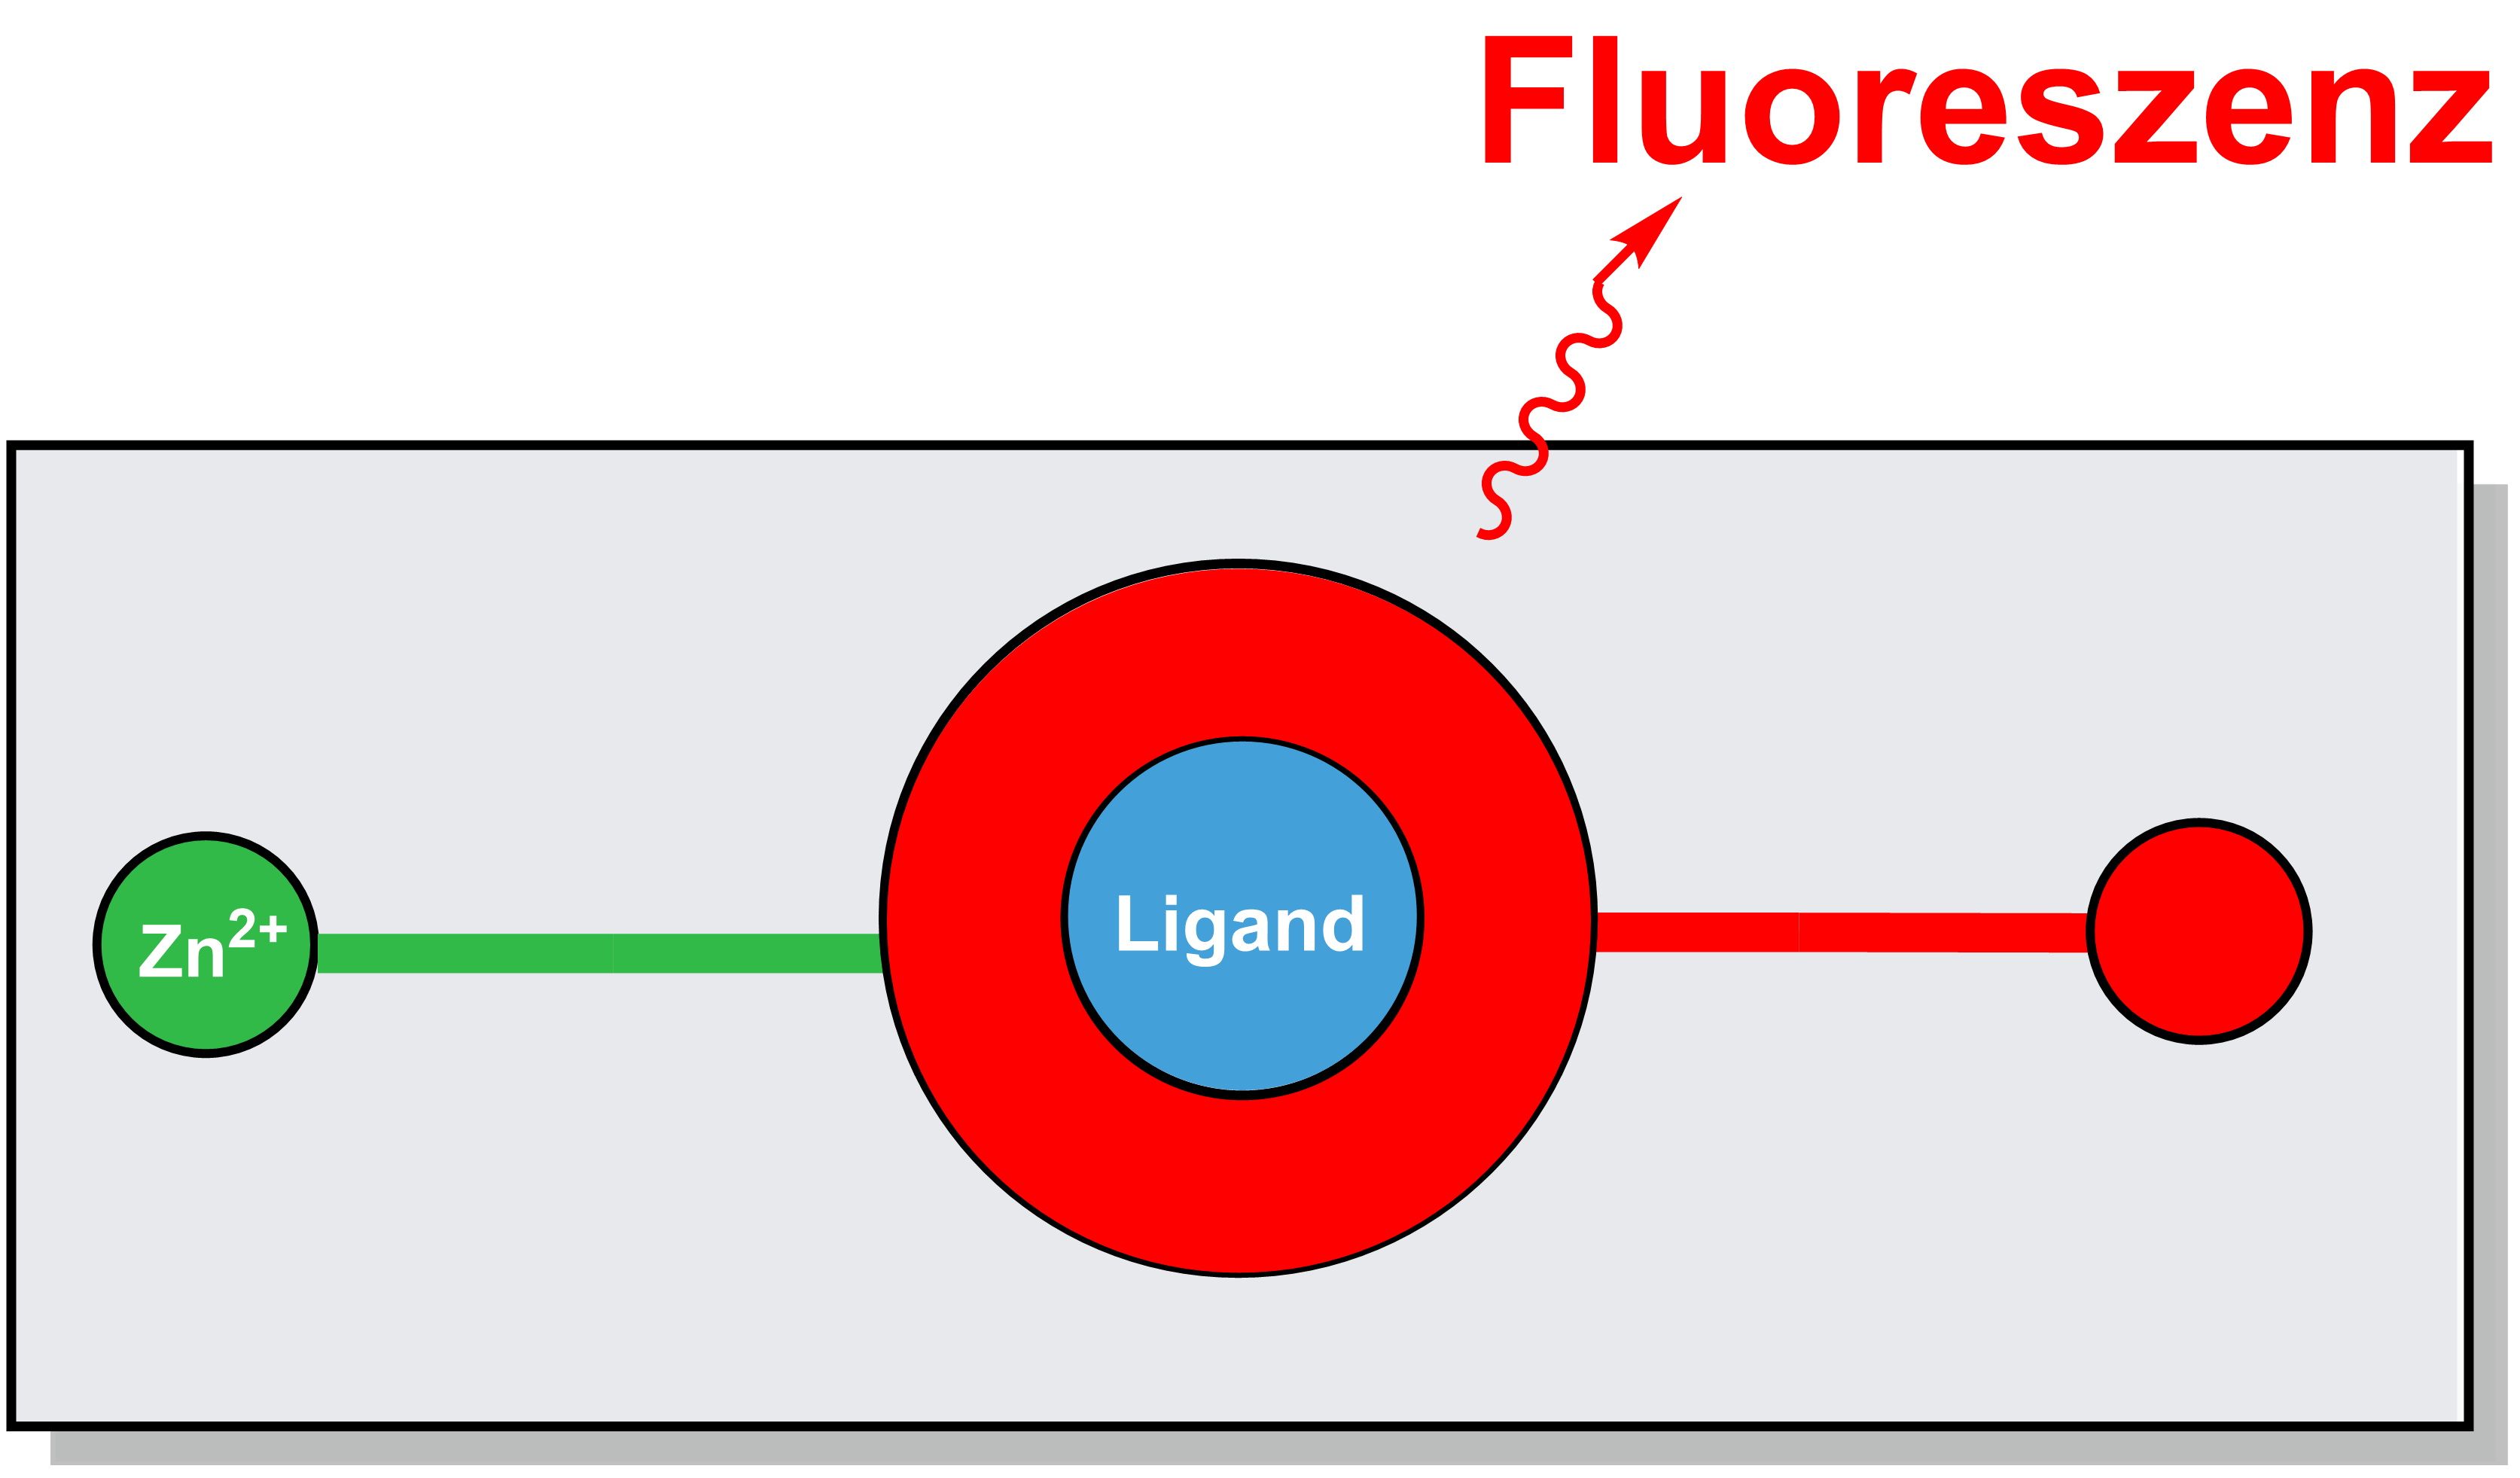
\includegraphics[width=0.5\textwidth]{Immobilisierung.png}
			\caption{\textnormal{\textit{Chipaubau beim Immobilisierungsansatz}.}}
			\label{fig:Immo}
		\end{figure}\\
	Der Flowansatz (\textbf{\autoref{fig:Flowansatz}}) benötigt je eine Lösung des Liganden und des Analyten. Dabei fließen beide Lösungen gleichzeitig durch den Chip, wobei der Komplex innerhalb der Mischkammer gebildet wird. 
	\begin{figure}[h!]
		\centering
		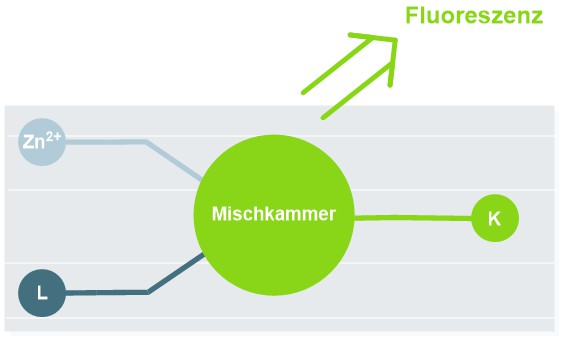
\includegraphics[width=0.5\textwidth]{Flowansatz.png}
		\caption{\textnormal{\textit{Chipaubau beim Flowversuch}.}}
		\label{fig:Flowansatz}
	\end{figure}
	\chapter{Ergebnisse und Diskussion}
	\section{Vorversuche am Modellsystem Pyranin}
	Da die Menge des Calix[4]arens begrenzt war, wurden zunächst Vorversuche zur Immobilisierung mit dem Fluoreszenzfarbstoff Trinatrium-8-hydroxypyren-1,3,6-trisulfonat (Pyranin) durchgeführt, dessen Fluoreszenzcharakteristika bereits in vielfältigen Veröffentlichungen dokumentiert wurden. Weitere Vorteile des Pyranins liegen in seiner Ungiftigkeit und der sehr guten Wasserlöslichkeit (bis zu 300 g$\cdot$\ce{l^{-1}}).\footnote{A. Herbst, H. Wygoda: Pyranin – ein fluoreszierender Farbstoff für
		applikationstechnische Versuche, Nachrichtenbl. Deut. Pflanzenschutzd., 58 (3), 2006, S. 79–85}
	\subsection{Spektroskopische Charakterisierung}
	%https://hal.archives-ouvertes.fr/hal-02991490/file/JCE_pyranine-Revisions-Final.pdf\\
	%file:///C:/Users/Olli/Downloads/10.1515_zna-1967-0923.pdf\\
	%https://www.bgu.ac.il/~epines/our%20papers%20PDF%20published/chemphyschem%20pines-nibbering.pdf
	%https://sci-hub.hkvisa.net/10.1039/c3cp53082e
	Es wurde ein UV/Vis-Absorptionsspektrum von Pyranin in Wasser im Wellenlängenbereich von 300 - 480 nm aufgenommen. Die spektroskopischen Charakteristika können \textbf{\autoref{tab:UVVisPyranin}} entnommen werden. 
	\begin{table}[h!]
		\centering
		\caption{\textnormal{\textit{Spektroskopische Merkmale des Pyranins in Wasser. Das Absorptionsspektrum lässt sich durch zwei Maxima charakterisieren.}}}
		\label{tab:UVVisPyranin}
		\begin{tabular}{p{2.5cm}p{2.5cm}l}
			\toprule
			Peak&$\mathbf{\uplambda_{max}}$/nm &\ce{A_{max}} \\ 
			\hline
			1&370&0,048\\
			2&404&0,058\\
			\bottomrule
		\end{tabular}
	\end{table}\\
	Das Absorptionsspektrum ist durch zwei Banden charakterisiert, welche sich im UV-B (370 nm) und im violetten Bereich des sichtbaren Lichtes befinden (404 nm). Letztere sorgt für die intensive gelbe Farbe des Pyranins.\\
	\ \\
	Die Absorptionsbande bei 370 nm lässt sich auf den \ce{S_0} $\rightarrow$ \ce{^1Lb}, die bei 400 nm auf den \ce{S_0} $\rightarrow$ \ce{^1La} Übergang zurückführen (\textbf{\autoref{fig:LaLb}}).\footnote{P. Changenet, T. Gustavsson, I. Lampre: Introduction to Femtochemistry: Excited State Proton Transfer from Pyranine to Water Studied by Femtosecond Transient Absorption, Journal of Chemical Education, 2020, S. 9} 
	Die Lage der Maxima  ist stark vom pH-Wert des Lösungsmittels abhängig (pKs = 7,4). Der Effekt ist auf die Deprotonierung der Hydroxygruppe (\textbf{\autoref{fig:StrukturPyranin}}) und der sich daraus ergebenden Erhöhung des +M-Effekts zurückzuführen. Dieser führt zu einem zunehmend bathochromen Shift der Peaks. Daher liegt das Absorptionsmaximum der deprotonierten Pyraninspezies bei 460 nm, und das der protonierten bei 404 nm.\footnote{S. K. Mondal, K. Sahu, P. Sen, D. Roy, S. Ghosh, K. Bhattacharyya: Excited state proton transfer of pyranine in a $\gamma$-cyclodextrin cavity, Chemical Physics Letters, 292, 2005, S. 229-230} Dem folgt, dass es sich im gemessenen Spektrum um die protonierte Form handelt.
		\begin{figure}[h!]
			\centering
			\includegraphics*[width=\textwidth]{PyraninpH.png}
			\caption{\textnormal{\textit{Struktur des Pyranins. Die OH-Gruppe übt einen bathochromen Effekt aus, welcher durch deren  Deprotonierung verstärkt wird.}}}
			\label{fig:StrukturPyranin}
		\end{figure}
			\begin{figure}[h!]
				\centering
				\includegraphics*[width=0.8\textwidth]{UVVisPyranin.jpg}
				\caption{\textnormal{\textit{UV/Vis-Absorptionsspektrum des Pyranins in Wasser im Wellenlängenbereich von 300-480 nm.} }}
				\label{fig:UVVisPyranin}
			\end{figure}\\
			\begin{figure}[h!]
				\centering
				\includegraphics*[width=0.4\textwidth]{LaLb.png}
				\caption{\textnormal{\textit{Für aromatische Moleküle können typischerweise zwei spektroskopisch zugängliche Zustände erreicht werden: Entweder mit Licht, das entlang der Bindungsachse (\ce{^1Lb}-Zustand) oder entlang der Atome (\ce{^1La}-Zustand) polarisiert ist.}}}
				\label{fig:LaLb}
			\end{figure}
	\noindent Es wurde ein Fluoreszenzspektrum des Pyranins bei einer Anregungswellenlänge von $\mathbf{\lambda}$\textbf{\ce{_{exc}}} = 420 nm in Wasser aufgenommen (\textbf{\autoref{fig:FluoreszenzPyranin}}). Das Emissionsmaximum liegt bei 506 nm und wird von der Literatur bestätigt.\footnote{K. A. Giuliano, R. J. Gillies: Determination of Intracellular pH of BALB/c-3T3 Cells Using the Fluorescence of Pyranine, Analytical Biochemistry, 1987, S. 365} Der verglichen mit dem Absorptionsspektrum bathochrome Shift des Emissionspeaks ist auf die typisch positive Solvatochromie des Pyranins zurückzuführen. Die Fluoreszenzlebensdauer (\textbf{\autoref{fig:FLDPyranin}}) liegt bei 1,14 s. \\
			\begin{figure}[h!]
				\centering
				\includegraphics*[width=0.8\textwidth]{FluoreszenzPyranin.jpg}
				\caption{\textnormal{\textit{Fluoreszenzspektrum des Pyranins in Wasser bei einer Anregungswellenlänge von 420 nm.}}}
				\label{fig:FluoreszenzPyranin}
			\end{figure}\\
			\begin{figure}[h!]
				\centering
				\includegraphics*[width=0.8\textwidth]{FLDPyranin.jpg}
				\caption{\textnormal{\textit{Die Fluoreszenzlebensdauer des Pyranins beträgt 1,14 ns.}}}
				\label{fig:FLDPyranin}
			\end{figure}\\
	\newpage
	\subsection{Immobilisierung}
		Nach der Immobilisierung zeigte das Pyranin zunächst zwei Emissionsmaxima im sichtbaren Bereich des elektromagnetischen Spektrums: Bei 440 nm und 509 nm. Dabei verschwindet der Peak bei 509 nm nach einer Spülung des Chips mit Wasser  (\textbf{\autoref{fig:PyraninFlow}}).\\
		\ \\
		\noindent Die Gruppe um \textnormal{Kızıldereli et al} beobachtete, dass eine  C-O-Bindung zwischen der Hydroxygruppe des Pyranins und dem terminalen C-Atom des Acrylamids eine hypsochrome Verschiebung im Emissionsspektrum des Pyranins verursacht. Gleichzeitig bewirken elektrostatische Wechselwirkungen zwischen den Sulfonsäuregruppen des Pyranins und den protonierten Amidgruppen der Acrylamidketten eine bathochrome Verschiebung des Peaks von 406 zu 430 nm.\footnote{N. Kızıldereli, A. Gelir, O. Güney, Y. Yılmaz: Theoretical Confirmation ofIn SituMonitoring ofMonomer Conversion During Acrylamide Polymerizationvia Pyranine Flouroprobe, Journal of Applied Polymer Science, 2009, S. 2456-2457} Dieser Effekt erklärt den Emissionspeak bei 440 nm.\\
		\ \\
		Das Emissionsmaximum bei 509 nm stimmt annähernd mit dem des Pyranins in Wasser überein. Da bei der Immobilisierung eine wässrige Lösung verwendet wurde, könnte dieser Peak auf ungebundenes Pyranin hindeuten. Diese Vermutung stimmt mit der Beobachtung überein, dass das Emissionsmaximum nach der Spülung verschwindet.\\
		\ \\
		Folglich lassen sich die beiden Maxima auf freies sowie immobilisertes  Pyranin zurückführen.
			\begin{figure}[h!]
			\centering 
			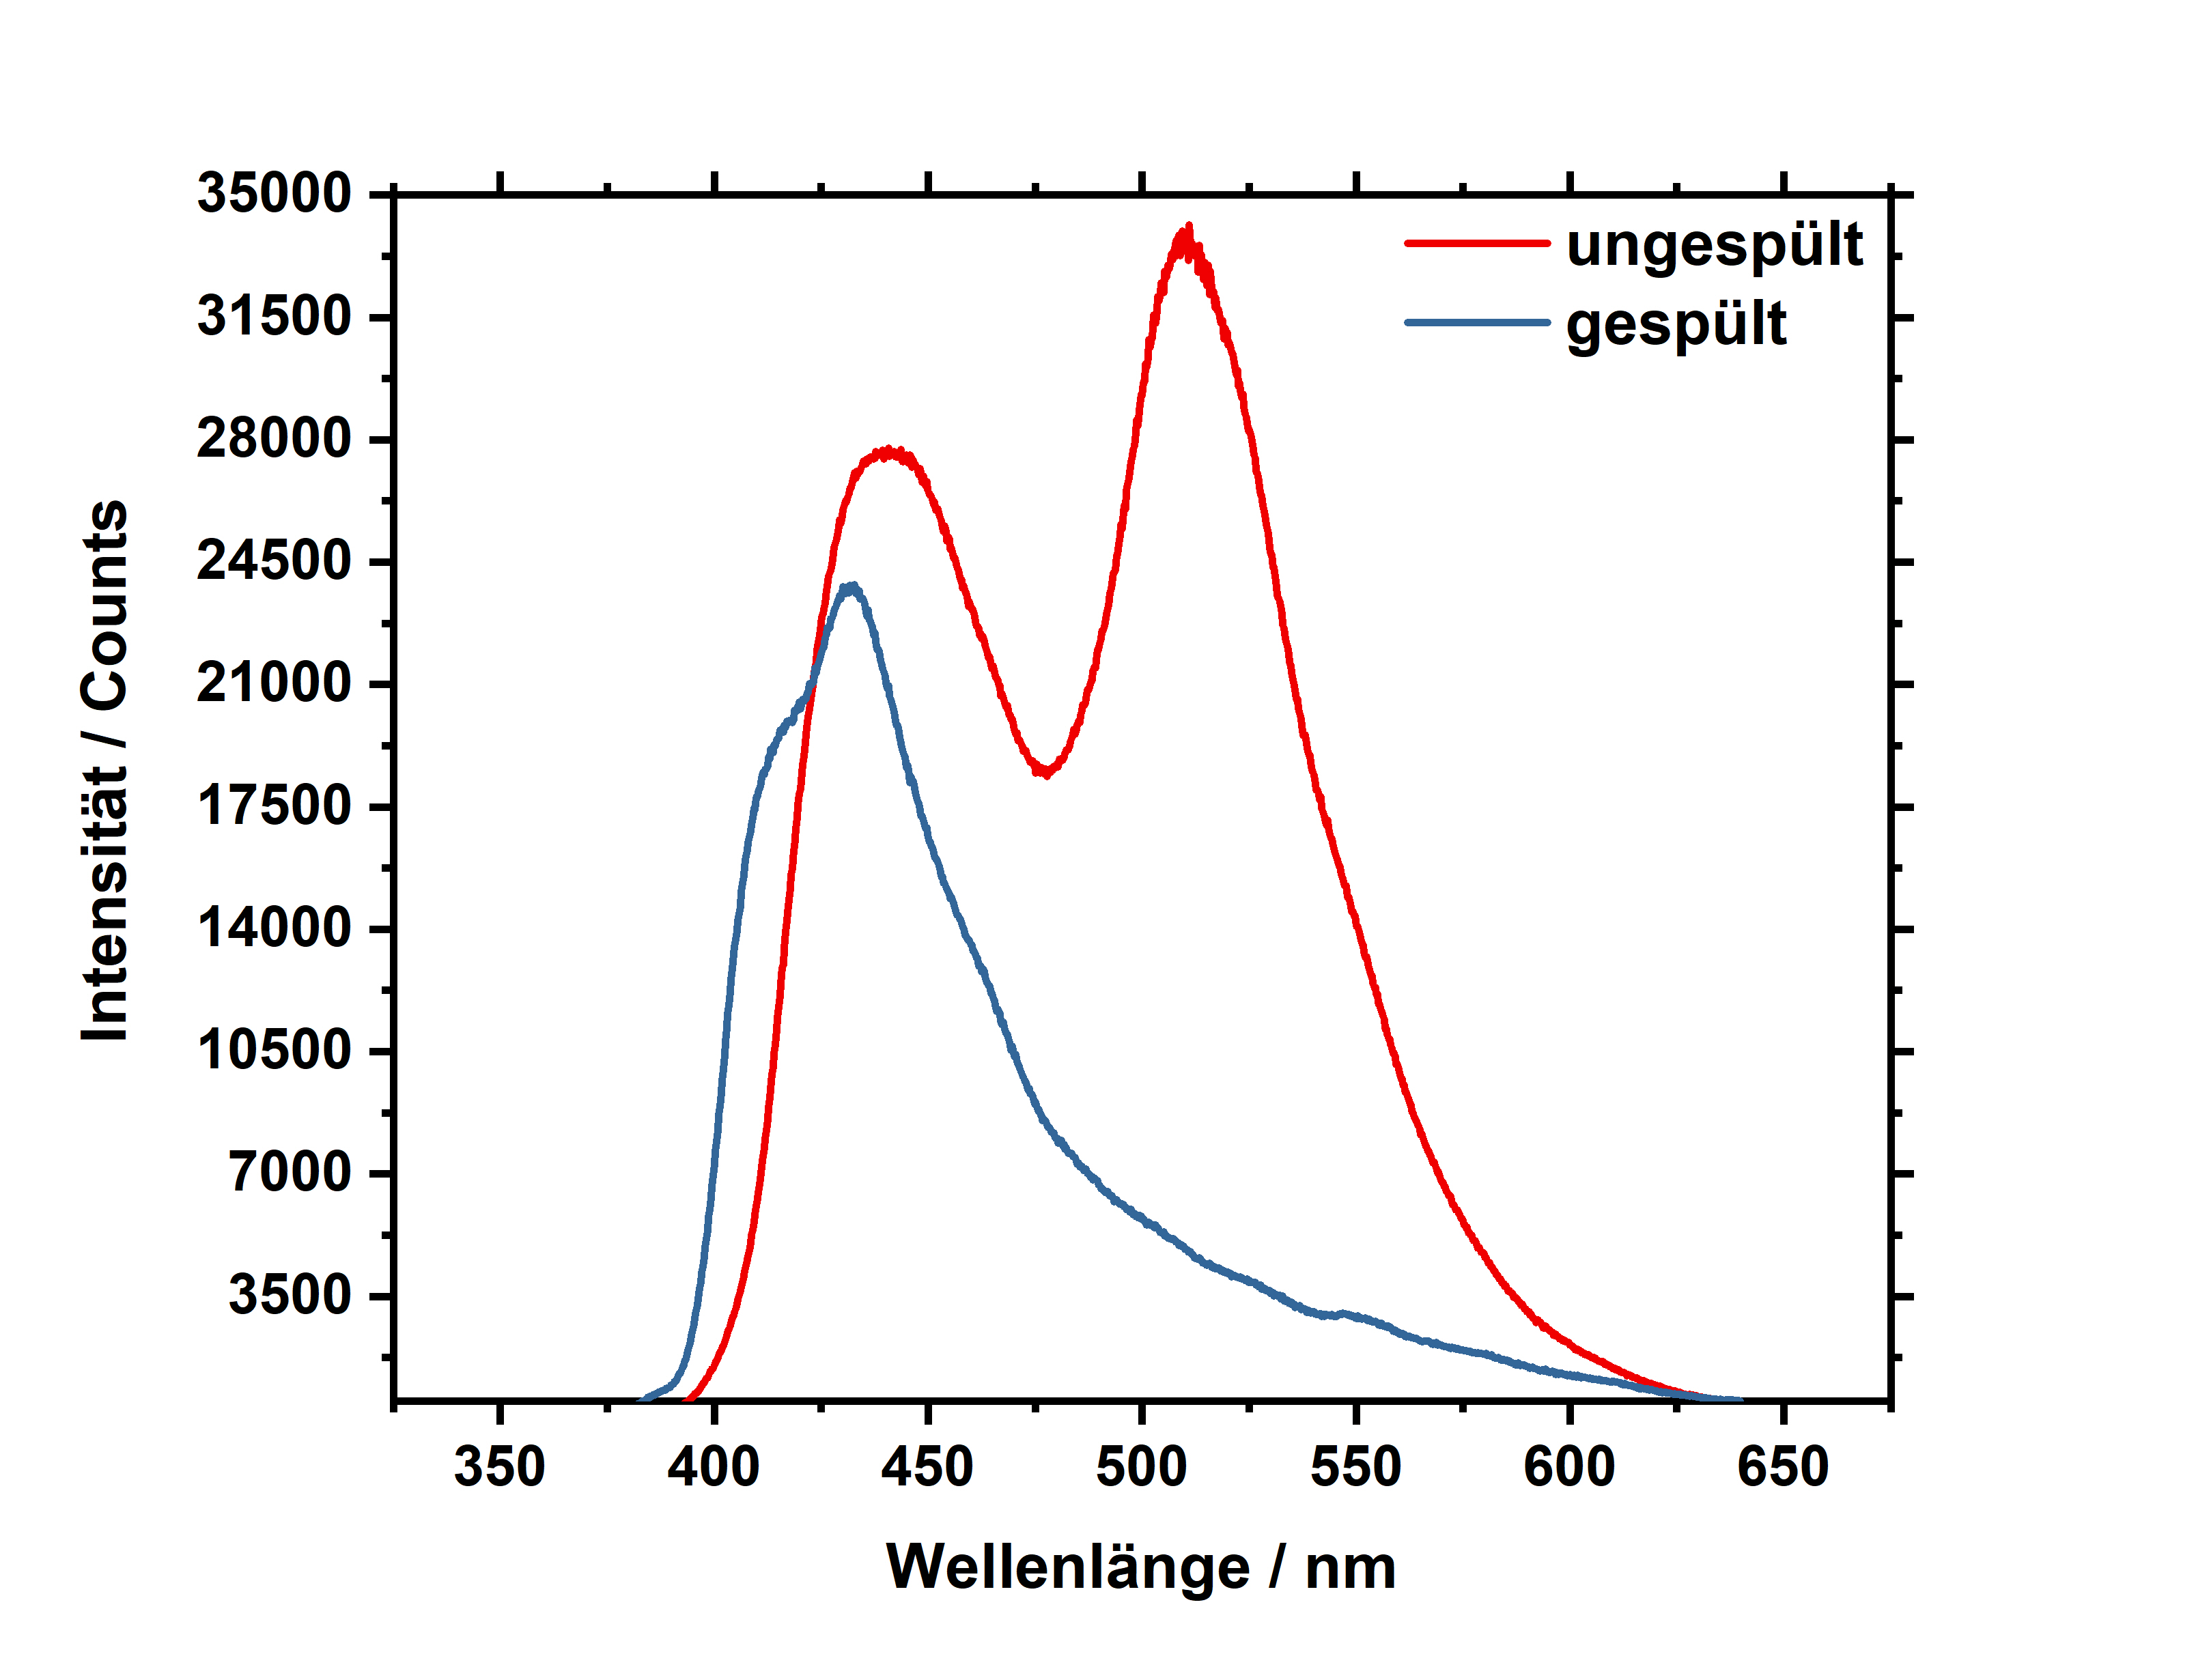
\includegraphics[width=0.8\textwidth]{ImmoPyranin.jpg}
			\caption{\textnormal{\textit{Fluoreszenzspektrum des immobilisierten Pyranins bei einer Anregungswellenlänge von 420 nm.}}}
			\label{fig:PyraninFlow}
			\end{figure} 
	\newpage 
	\section{Calix[4]aren}
	\subsection{Studie zur Fähigkeit als Zinkdetektor}
	Es wurde ein UV/Vis-Absorptionsspektrum des reinen Calixarens (\textbf{\autoref{fig:Calixaren}}) sowie des Calixarens unter Zugabe von Zinkacetat aufgenommen (\textbf{\autoref{fig:UVVISLigandKomplex}}). Die spektroskopischen Merkmale können \textbf{\autoref{tab:UVVisLigandKomplex}} entnommen werden.
		\begin{table}[h!]
			\centering
			\caption{\textnormal{\textit{Spektroskopische Merkmale und verwendete Konzentrationen des Liganden sowie des Zinkkomplexes in Ethanol.}}}
			\label{tab:UVVisLigandKomplex}
			\begin{tabular}{p{2.5cm}p{2.5cm}p{2.5cm}p{2.5cm}l}
				\toprule
				Spezies&c/\textmu M&Peak&$\mathbf{\uplambda_{max}}$/nm &\ce{A_{max}} \\ 
				\hline
				Ligand&3,75&1&263&0,048\\
					  &    &2&328&0,0072\\
				\hline 
				Komplex&0,008&1&260&0,1397\\
					   &     &2&330&0,0294\\
				\bottomrule
			\end{tabular}
		\end{table}\\
	Die Form der Absorptionsbanden scheint für beide Spezies nahezu identisch. Die Wellenlängendifferenz zwischen den Peaks des Liganden und des Komplexes ist vernachlässigbar gering. Beide Spektren besitzen ein  Absorptionsmaximum bei 260 nm sowie eine zweite Absorptionsbande geringerer Intensität im längerwelligen Bereich bei 330 nm, welche auf $\pi \rightarrow \pi^*$ Übergänge zurückgeführt werden können.\\
	\ \\
	Der markante Unterschied zwischen den Spektren liegt in der Intensität der Banden: Trotz der bei weitem geringeren Konzentration des Komplexes (\ce{c_{Komplex}} = 0,008 \textmu M ggü. \ce{c_{Ligand}} = 3,75 \textmu M) ist die Intensität der ihm zugehörigen Absorptionsbanden deutlich erhöht.\\
	\ \\ 
	Die gleiche Beobachtung ergibt sich in Bezug auf die Fluoreszenzspektren der beiden Spezies (\textbf{\autoref{fig:FluoreszenzLigandKomplex}}). Hier liegt das Emissionsmaximum von Ligand und Komplex bei jeweils 468 nm, jedoch ist die Intensität des Komplexes bei gleicher Konzentration etwa doppelt so hoch. 
	\newpage 
		\begin{figure}[h!]
			\centering 
			\includegraphics[width=0.8\textwidth]{UVVIsLigandKomplex.jpg}
			\caption{\textnormal{\textit{Absorptionsspektrum des Liganden (rot, c = 3,75 \textmu mol \ce{L^{-1}}) und des Komplexes (blau, c = 0,008 \textmu mol \ce{L^{-1}}) in Ethanol im Wellenlängenbereich von 290 - 480 nm.}}}
			\label{fig:UVVISLigandKomplex}
		\end{figure}
		\begin{figure}[h!]
			\centering 
			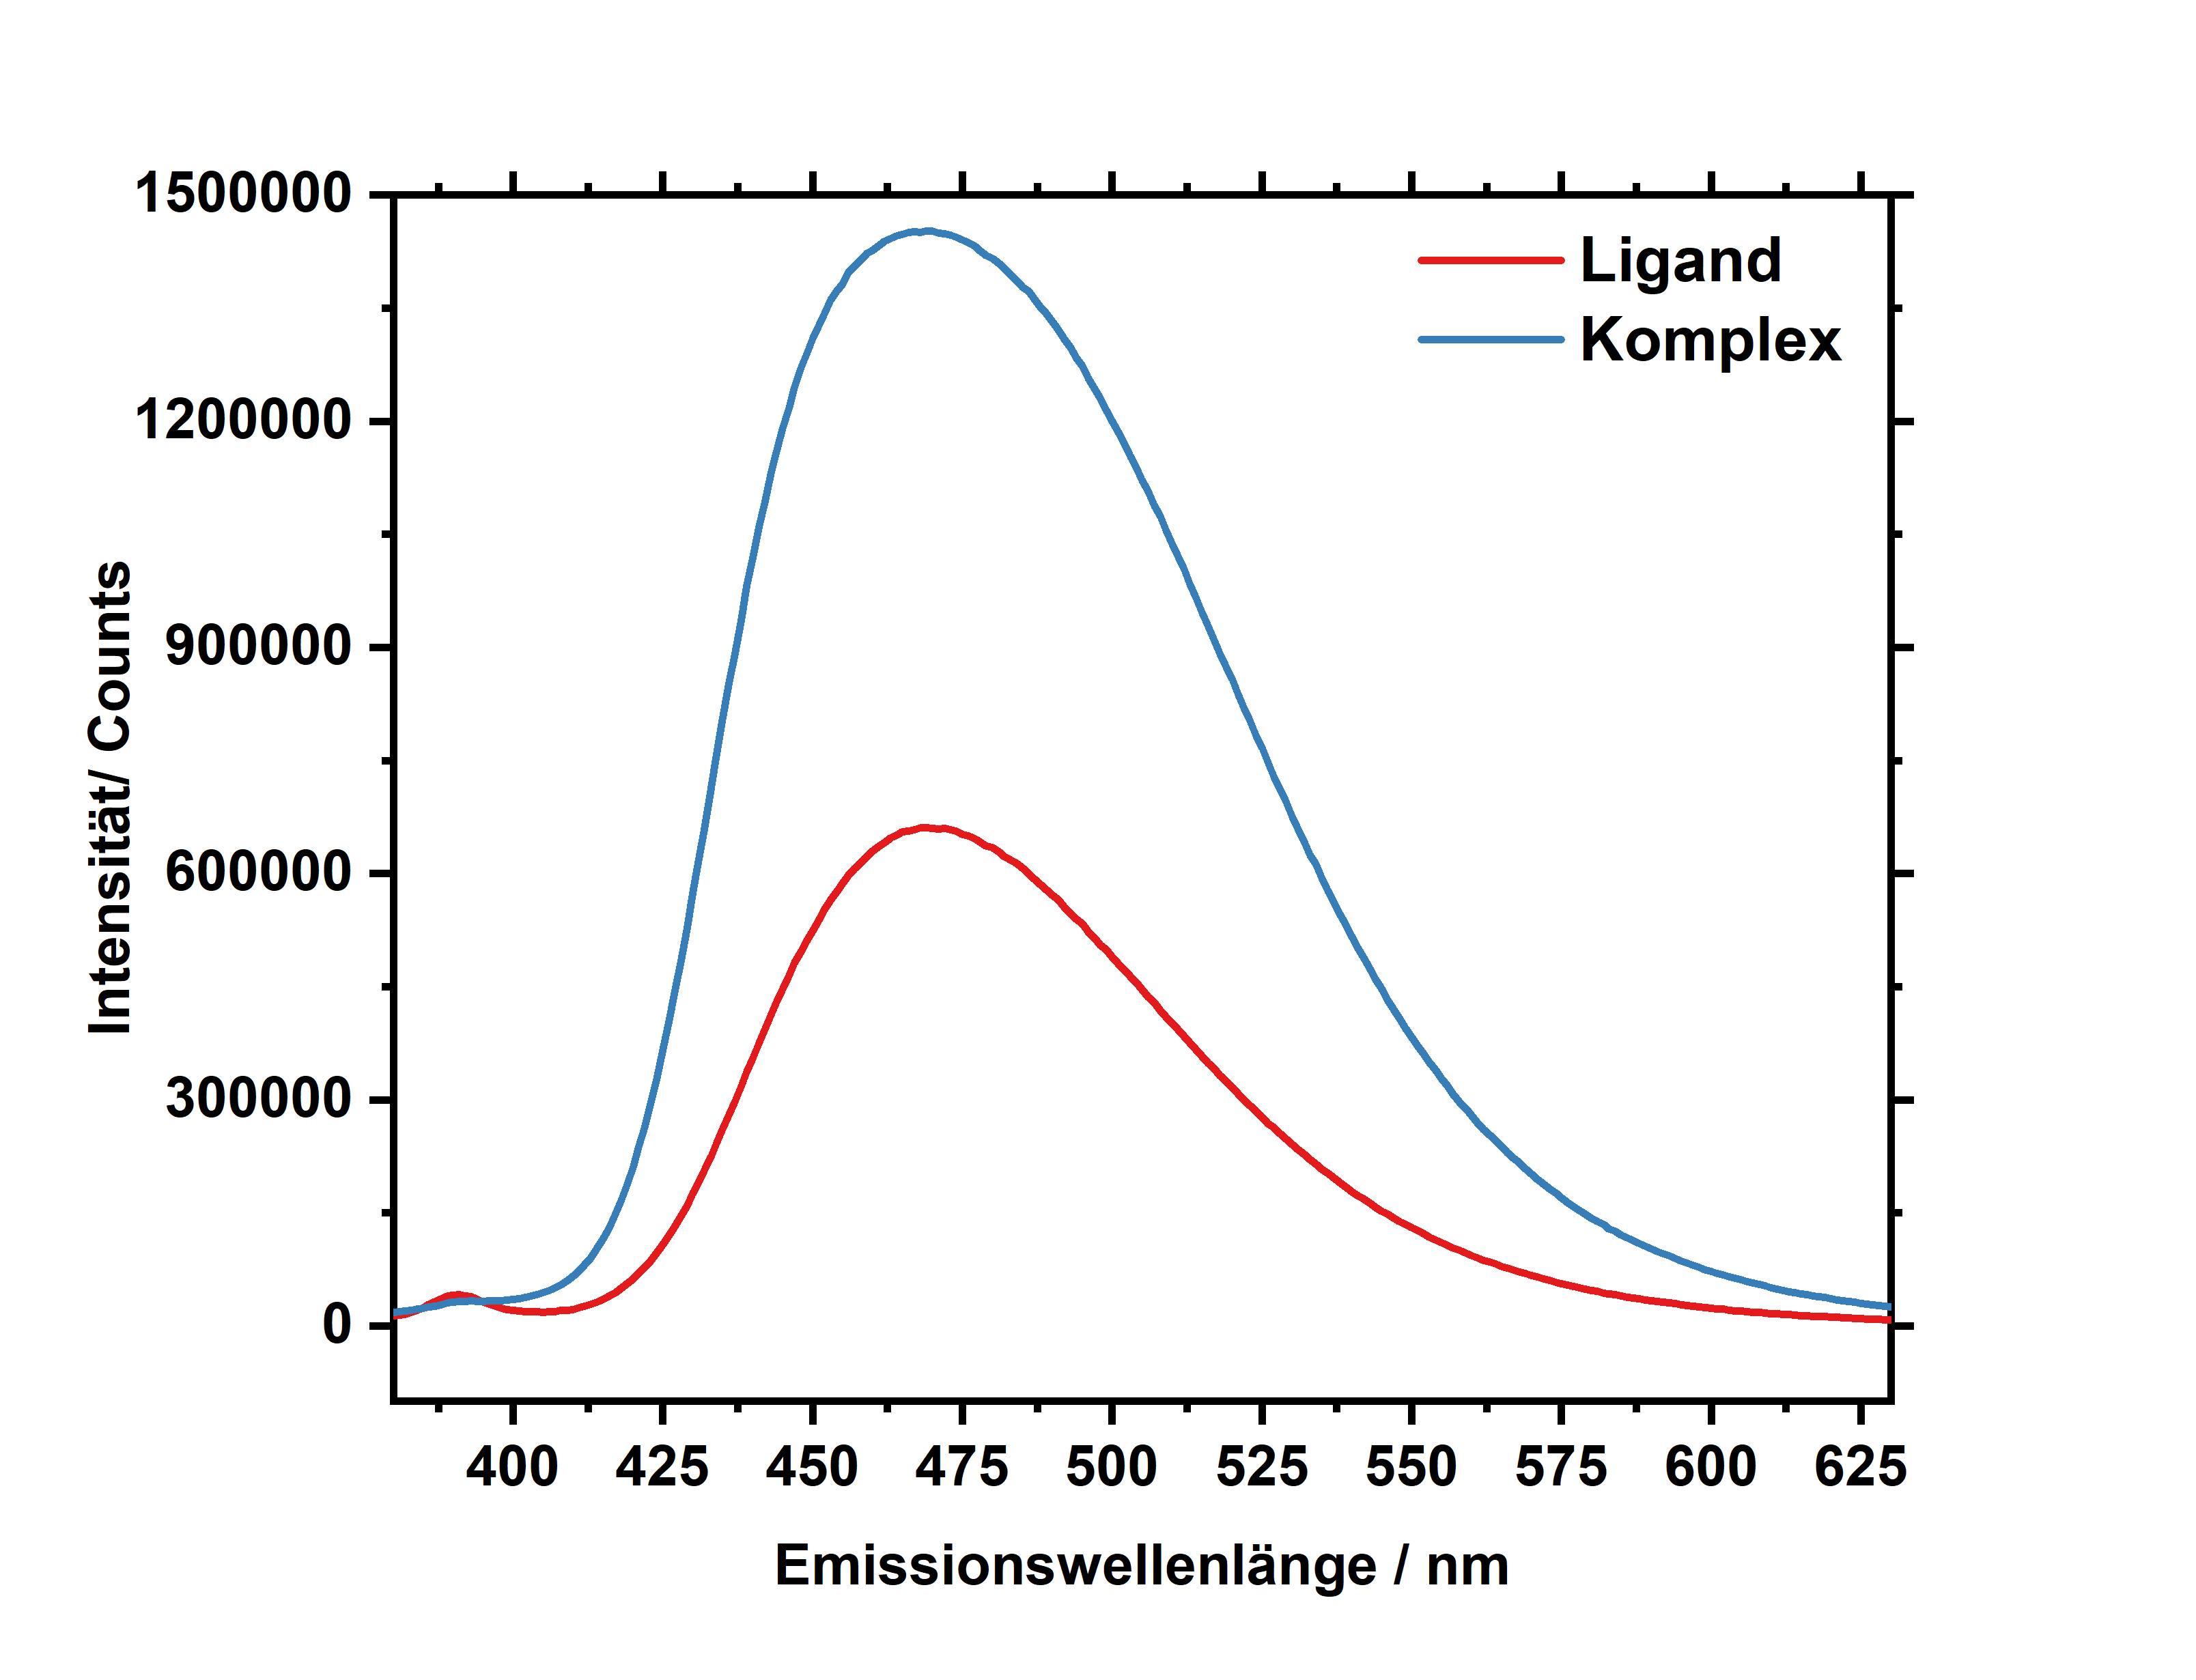
\includegraphics[width=0.8\textwidth]{FluoreszenzLigandKomplex.jpg}
			\caption{\textnormal{\textit{Emissionsspektrum des Liganden (rot, c = 3,75 \textmu mol \ce{L^{-1}}) und des Komplexes (blau, c = 0,008 \textmu mol \ce{L^{-1}}) in Ethanol im Wellenlängenbereich von 240 - 380 nm.}}}
			\label{fig:FluoreszenzLigandKomplex}
		\end{figure}
	\newpage 
	\noindent Die niedrige Fluoreszenz des freien Liganden ist sowohl auf den PET-Prozess, als auch auf die C=N-Isomerisierung der Schiffschen Base zurückzuführen. Durch die Zugabe der \ce{Zn^{2+}}-Ionen tritt ein CHEF-Effekt ein, welcher zum Anstieg der Fluoreszenz im Komplex führt. 
		\begin{figure}[h!]
			\centering 
			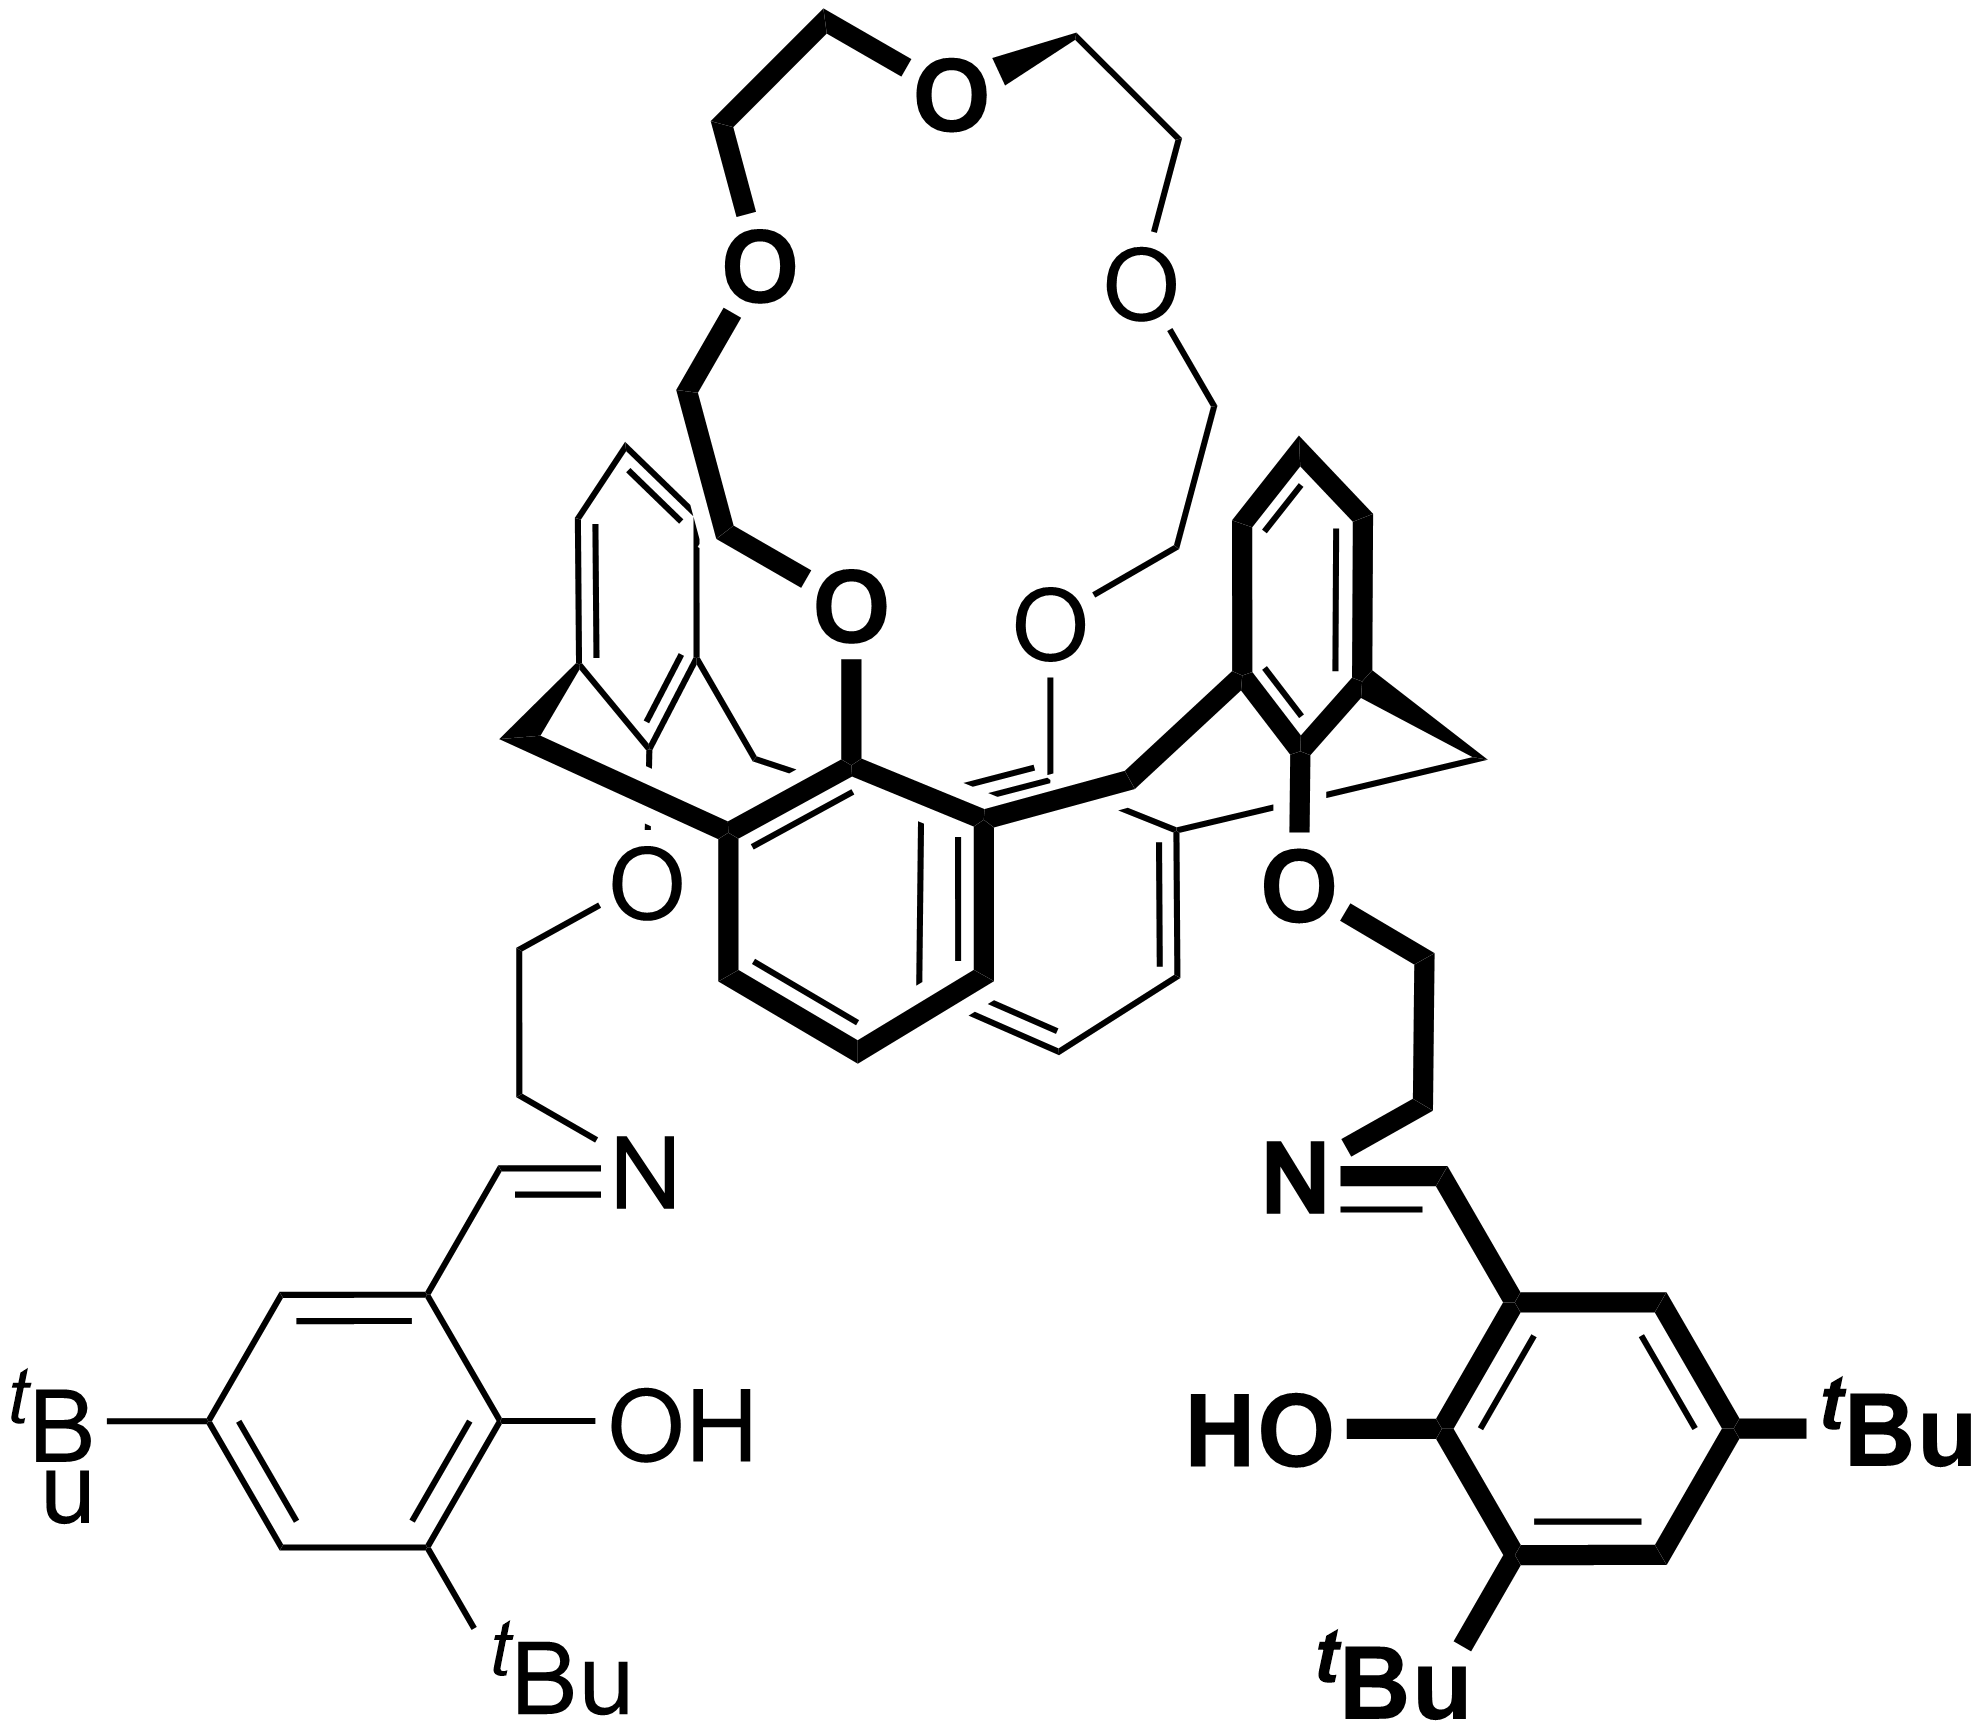
\includegraphics[width=0.5\textwidth]{Calixarenligand.png}
			\caption{\textnormal{\textit{Struktur des Calixarens.}}}
			\label{fig:Calixaren}
		\end{figure}\\
	Die Fluoreszenzlebensdauer des Calixarens liegt bei 3,01 ns und ist damit höher als die des Komplexes (1,04 ns). 
		\begin{figure}[h!]
			\centering 
			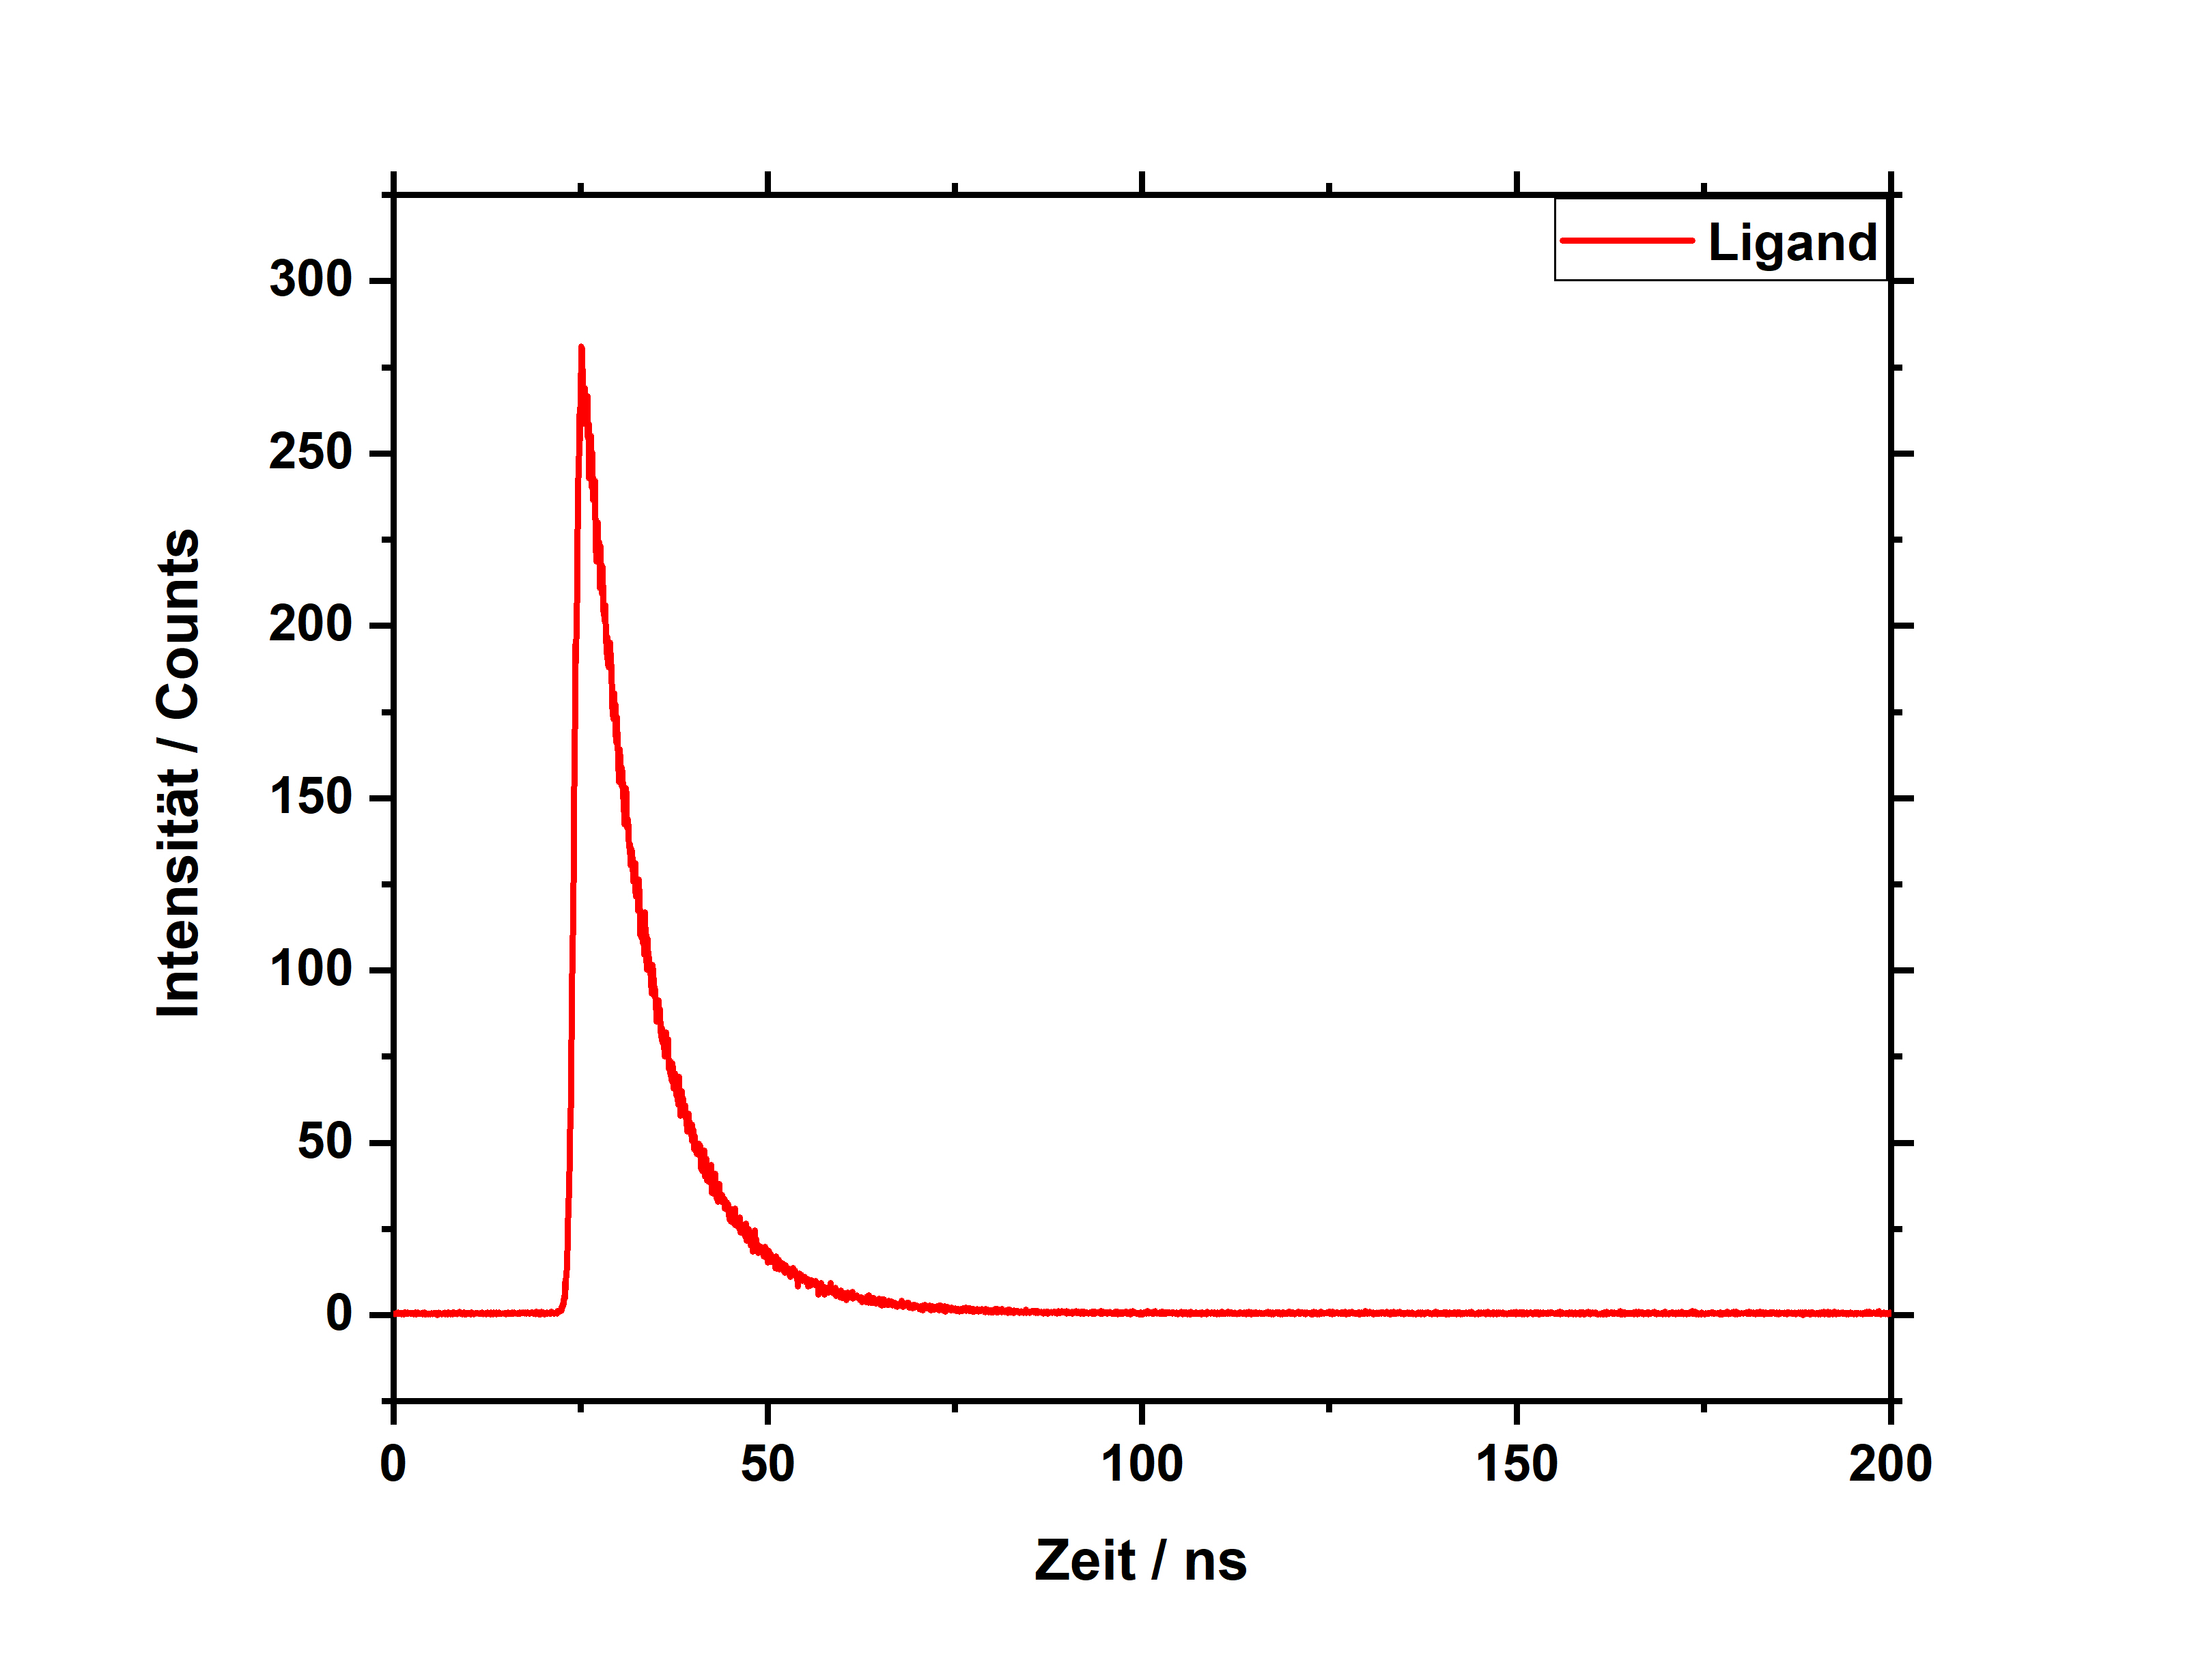
\includegraphics[width=0.8\textwidth]{FLDLigand.jpg}
			\caption{\textnormal{\textit{Die Fluoreszenzlebenszeit des Calixarens liegt bei 3,01 ns}}}
			\label{fig:FLDCalixaren}
		\end{figure}
		\begin{figure}[h!]
			\centering 
			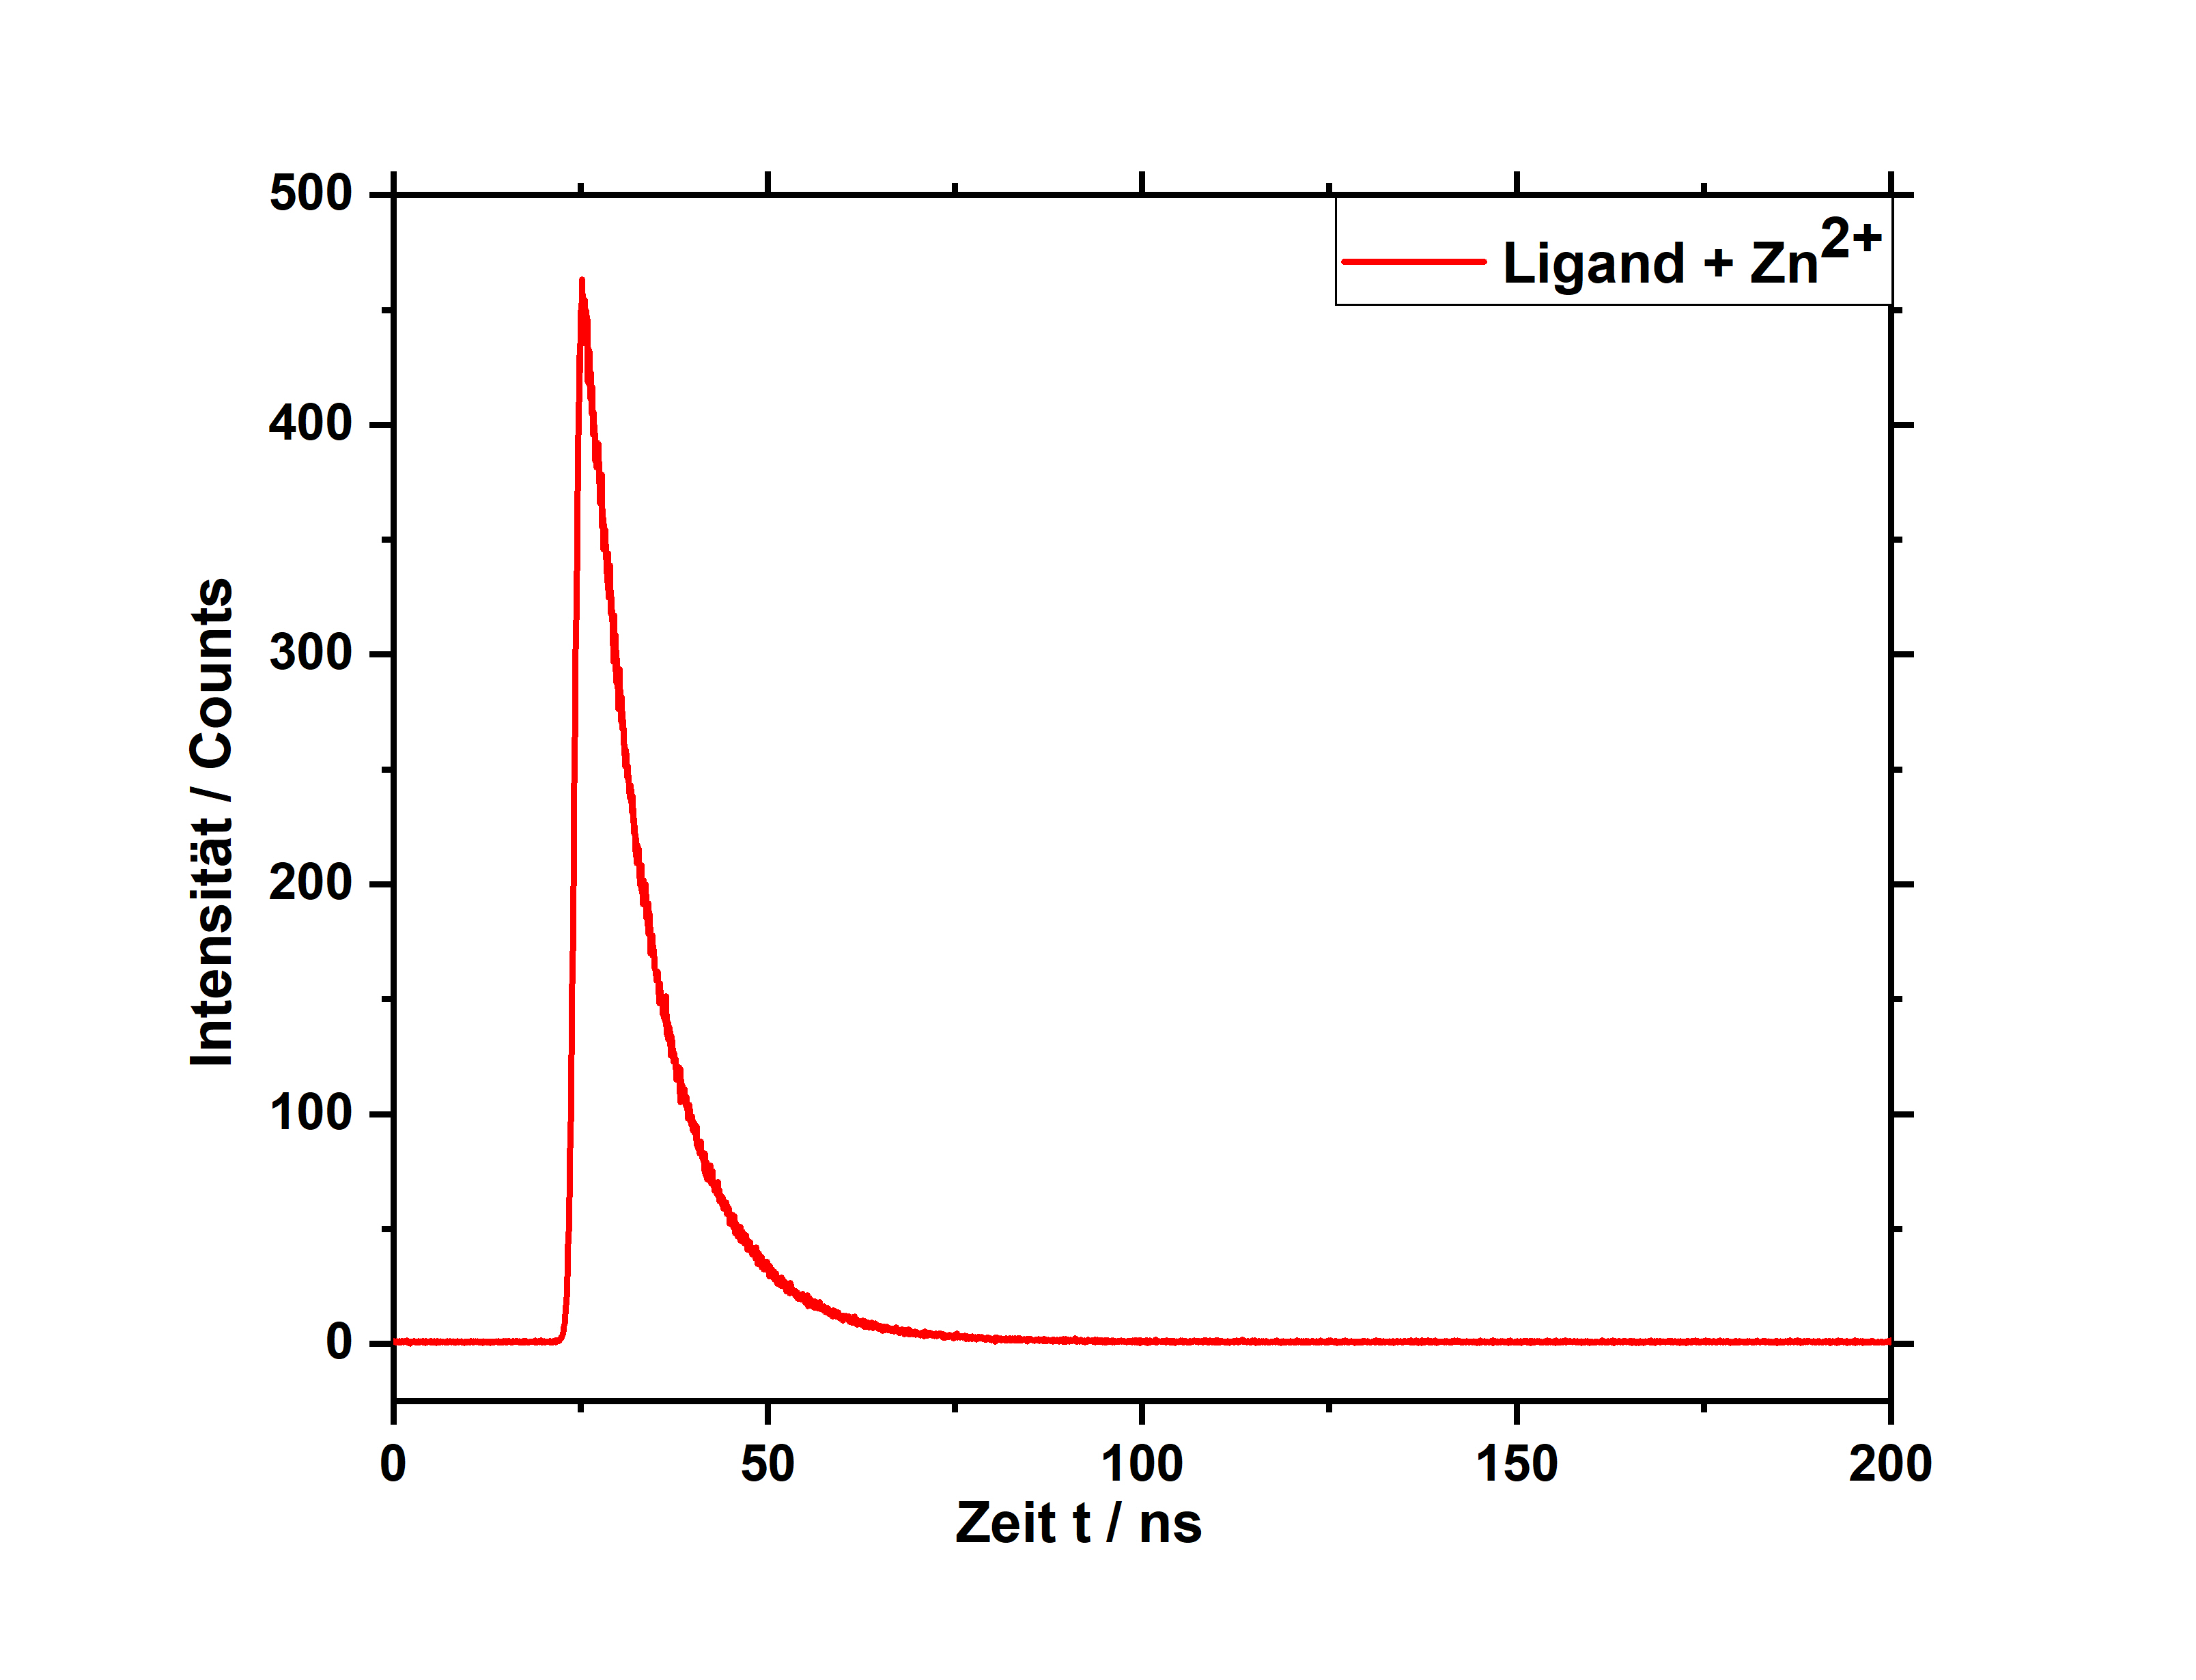
\includegraphics[width=0.8\textwidth]{FLDLigandZn.jpg}
			\caption{\textnormal{\textit{Die Fluoreszenzlebenszeit des Komplexes liegt bei 1,13 ns.}}}
			\label{fig:FLDKomplex}
		\end{figure}
	
	\subsection{Immobilisierung}
	Zur Durchführung der Immobilisierung war es zunächst notwendig, das Calixaren in Wasser zu lösen. Dies gelang aufgrund der schlechten Löslichkeit des Liganden nur in äußerst geringen Konzentrationen (c = 2,22 \ce{10^{-5}} M). Das aufgenommene Spektrum zeigt keine Fluoreszenz.\\
	\ \\
	Zur Verfolgung dieses Ansatzes ist demnach ein anderer Ligand notwendig. Eine andere Möglichkeit wäre den Chipdruck unter Verwendung von Ethanol durchzuführen, was allerdings aufgrund seines geringen Gefrierpunktes (-114,1 \textdegree C)\footnote{RÖMPP-Redaktion: Ethanol, (2019) in Böckler F., RÖMPP [Online], Stuttgart, Georg Thieme Verlag, [Oktober 2022]} nicht im Umfang dieser Arbeit betrachtet werden konnte. 
	\newpage 
	\subsection{Flowansatz}
	Der Flowansatz wurde mit einer Durchflussgeschwindigkeit von 70 \textmu L $\cdot$ \ce{min^{-1}} für beide Lösungen durchgeführt. Innerhalb der Mischkammer konnte mit wachsendem Weg eine steigende Fluoreszenz beobachtet werden. Die Komplexierung und die damit verbundene Fluoreszenz wird vom aufgenommenen Spektrum bestätigt. Das Emissionsmaximum des Komplexes liegt bei 484 nm und ist demnach gegenüber der wässrigen Lösung bathochrom verschoben. Die Zunahme der Intensität ist bei der Verwendung gleichmolariger \ce{Zn^{2+}}- und Calix[4]arenlösungen um das 16-fache erhöht. Durch den  Vergleich mit der spektroskopischen Charakterisierung des Liganden, bei der lediglich eine Verdopplung der Fluoreszenzintensität festgestellt wurde, kann von einer Abhängigkeit zwischen der Zinkkonzentration und der Fluoreszenzintensität ausgegangen werden. 
		\begin{figure}[h!]
			\centering 
			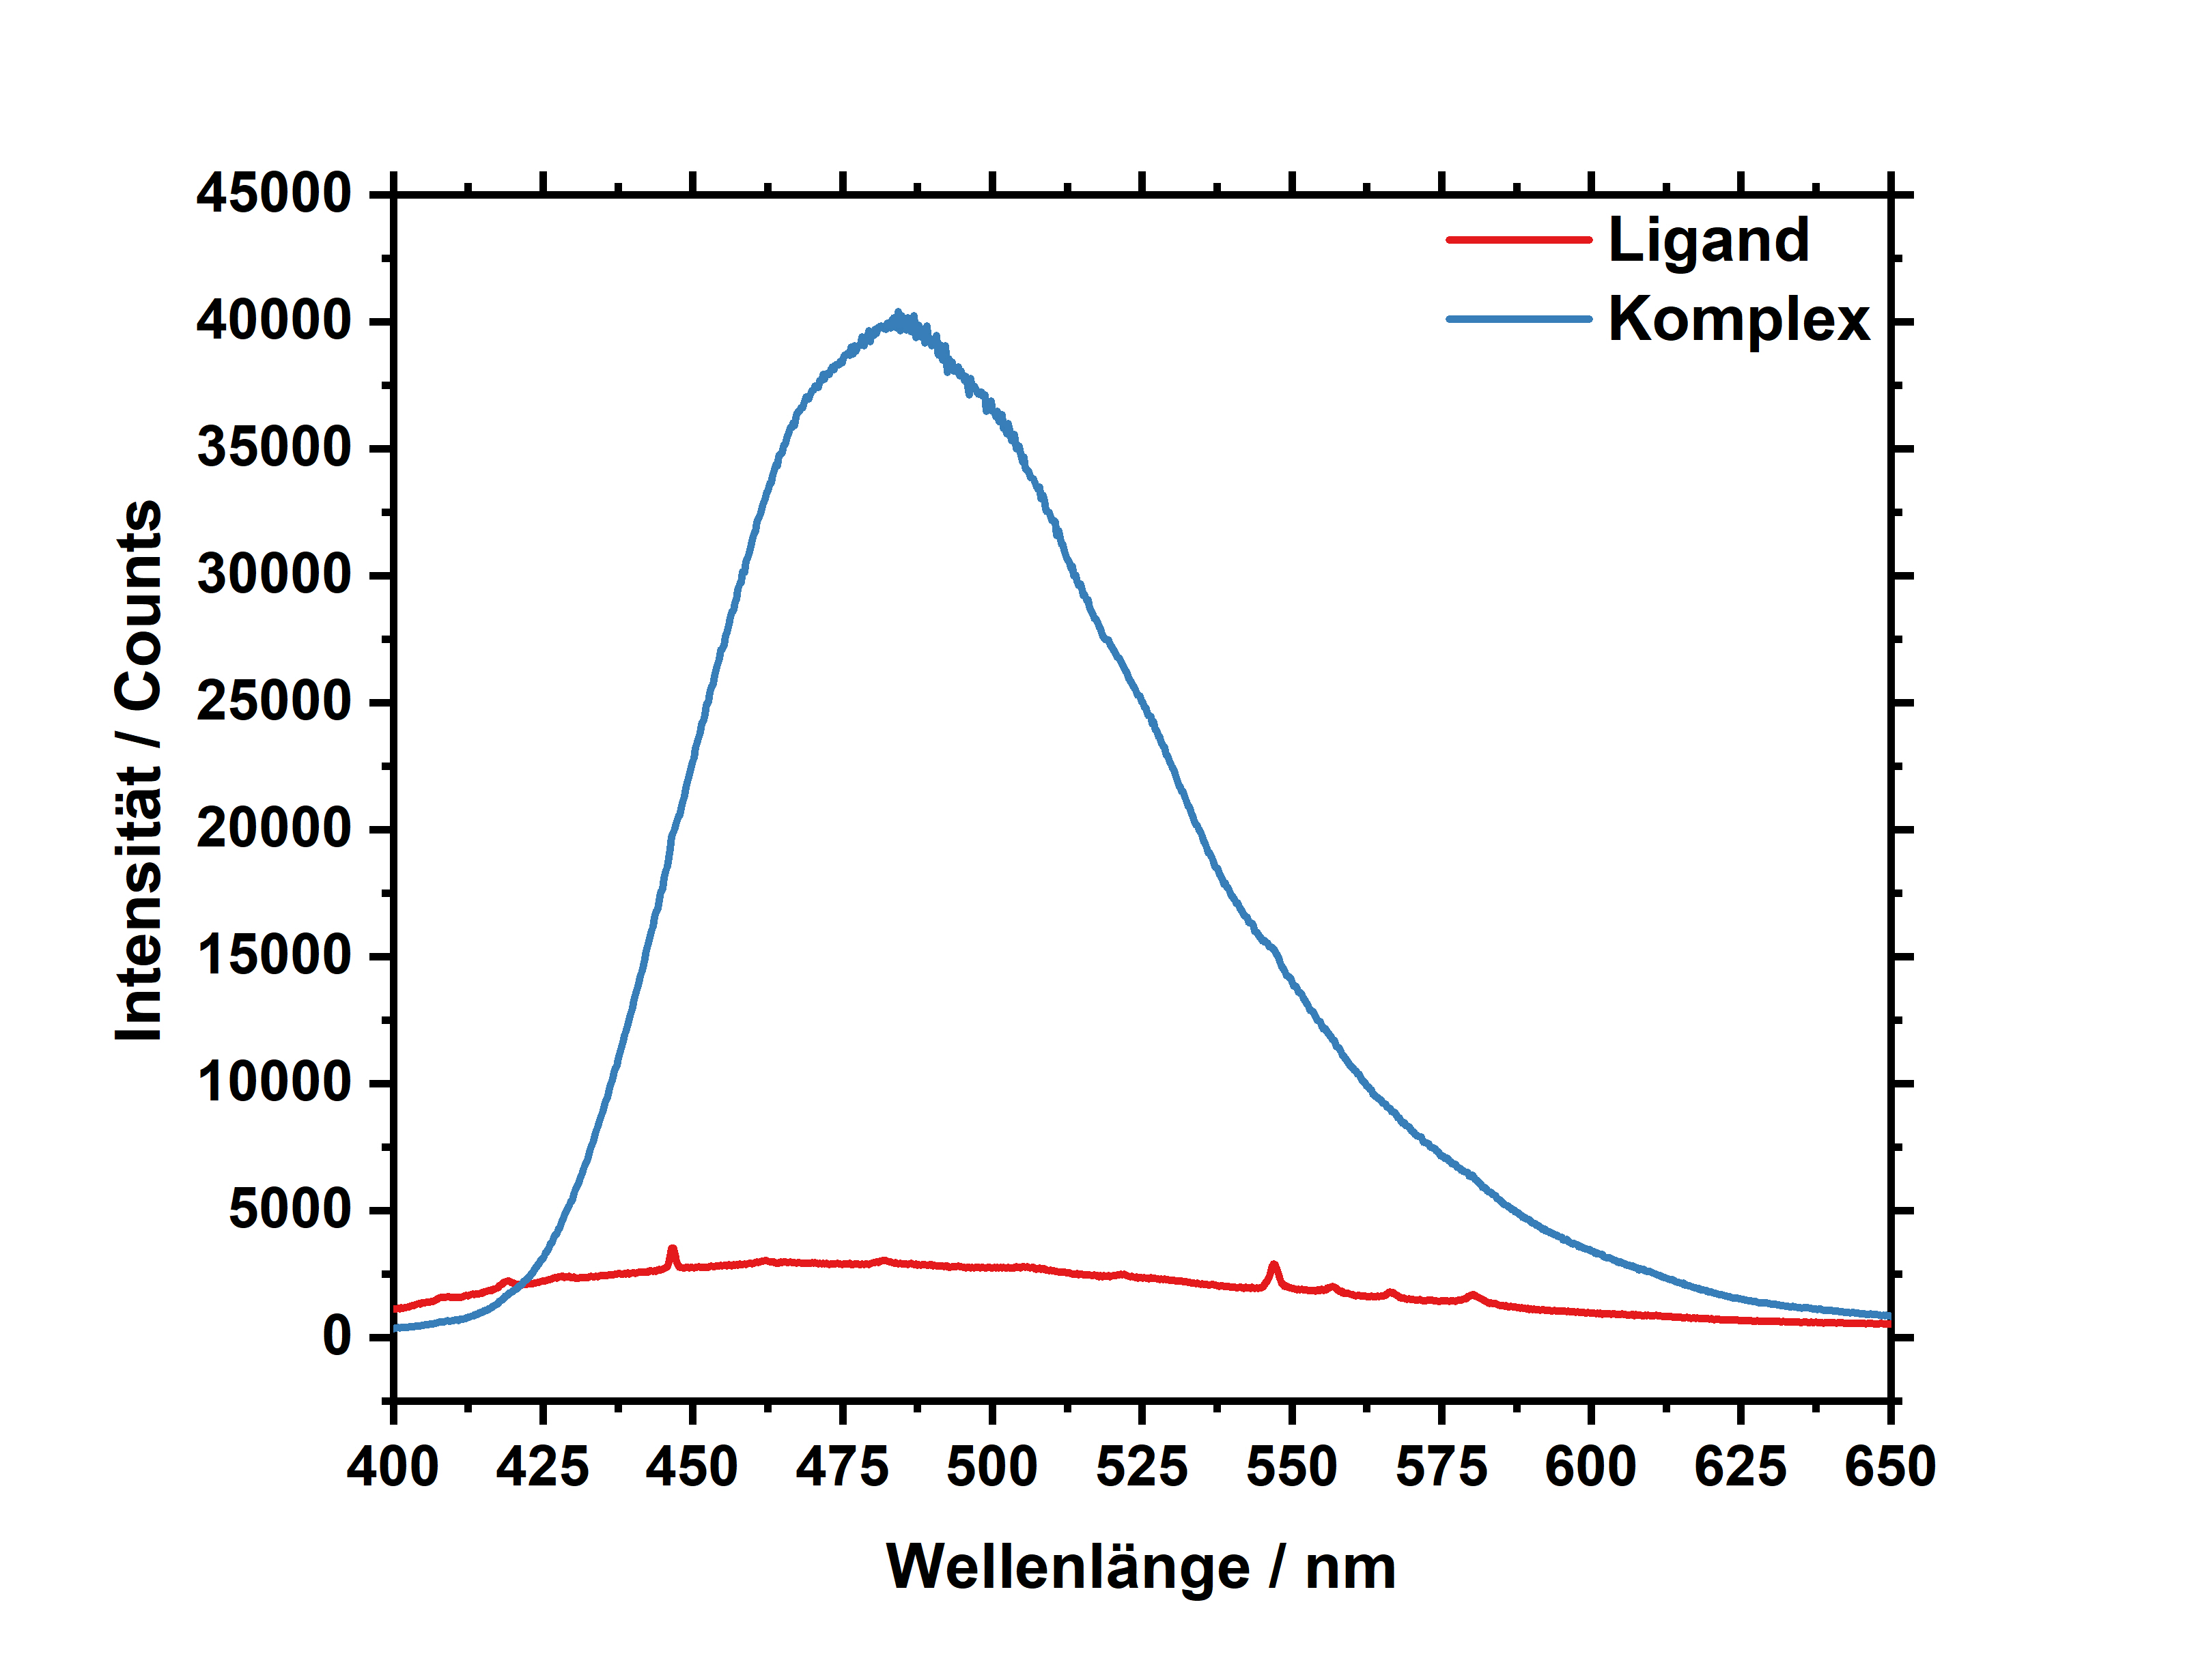
\includegraphics[width=0.8\textwidth]{FlowLigandKomplex.jpg}
			\caption{\textnormal{\textit{Fluoreszenzspektrum des Liganden und des Komplexes in Ethanol im Wellenlängenbereich von 400 - 650 nm.}}}
			\label{fig:FlowLigandKomplex}
		\end{figure}
	\chapter{Ausblick}
	\noindent Es konnte gezeigt werden, dass der Calix[4]arenligand als PET-Sensor für \ce{Zn^{2+}} geeignet ist. Dabei wurde jedoch keine Überprüfung der Selektivität, welche sich oftmals insbesondere in Bezug auf \ce{Cd^{2+}} als problematisch erweist, durchgeführt. Die Ursache liegt in der ähnlichen elektronischen Struktur der beiden Kationen. Auch die Konzentrationsgrenzen innerhalb derer die Zinkionen detektierbar sind, müssen den Gegenstand weiterer Arbeiten bilden.\\
	\ \\
	In Bezug auf die Miniaturisierung mittels Lab on a chip-Techniken scheint der Flowansatz erfolgversprechend. Bei Einsatz gleichmolarer Lösungen konnte eine Erhöhung der Fluoreszenzintensität um das 16-fache beobachtet werden. Durch eine Studie der Fluoreszenzintensität in Abhängigkeit von der Zinkkonzentration könnte die Stöchiometrie des Komplexes untersucht werden. \\
	\ \\
	Die Immobilisierung konnte dagegen bislang nicht durchgeführt werden. Hier könnten Untersuchungen mit wasserlöslichen Calix[4]aren Zinksensoren einen weiteren Forschungsansatz bieten. So gelang der Gruppe um Erdemir et al die Synthese eines wasserlöslichen Fluoreszenzsensors, welcher im unteren Ring des Calix[4]arens Phenolphthalein integriert.\footnote{S. Erdemir, S. Malkondu, O. Kocyigit: A reversible calix[4]arene armed phenolphthalein based fluorescent probe for the detection of Zn2+ and an application in living cells, Luminescence, 2018, S. 1}
	\chapter{Experimenteller Teil}
	\section{Spektroskopische Charakterisierung}
	Alle Lösungen wurden mittels Fluoreszenzspektroskopie auf Unreinheiten überprüft. Beim verwendeten Spektralfluorometersystem handelte es sich um \textit{FluoroMax - 4} mit der zugehören\textit{ FluorEssence} Software (V 3.9). \\
	\ \\
	Die Aufnahme der UV/Vis-Absorptionsspektren erfolgte über das Zweistrahlphotometer \textit{Shimadzu UV-2101 PC} und der \textit{UV-2102 PC} Software.
	\section{Chipdruck}
	Der Templatdruck erfolgt mit Wasser auf einem gekühlten silanisierten Träger unter Stickstoffatmosphäre. Die Zusammensetzung des Acrylats ist in \textbf{\autoref{tab:Acrylat}} aufgelistet. 
	\begin{table}[h!]
		\centering
		\caption{\textnormal{\textit{Zusammensetzung des Acrylats.}}}
		\label{tab:Acrylat}
		\begin{tabular}{p{4.5cm}p{4.5cm}l}
			\toprule
			Substanz&Masse / g & Aufgabe\\
			\hline 
			Isobornylacrylat (LBCA) & 7& Grundgerüst\\
			Ebecryl 40 (Ebe 40)&1,5& Haftvermittler\\
			Sartomer 285 (SR 285)&1& Haftvermittler\\
			Ebecryl 170(Ebe 170)&0,5 &Haftvermittler\\
			Omirad TPO-L (Tpol) & 0,1 &Photoinitiator\\
			\bottomrule
		\end{tabular}
	\end{table}\\
	Zur Immobilisierung wurde eine Spatelspitze Pyranin in 1,00 g Kryogel gelöst und mit 2,00 g \ce{H_2O} verdünnt. Die Lösung wurde über 0,45 \textmu m Poren gefiltert. Die Zusammensetzung des Kryogels kann \textbf{\autoref{tab:Kryogel}} entnommen werden. 
	\begin{table}[h!]
		\centering
		\caption{\textnormal{\textit{Zusammensetzung des Kryogels.}}}
		\label{tab:Kryogel}
		\begin{tabular}{p{9.5cm}l}
			\toprule
			Substanz&Masse / g\\
			\hline
			Polyethylendigklykol acrylat(PEG 60 A Mb700) & 1,00\\
			n-Isopropylacrylamid (NIPAAm) & 0,25\\
			Esacure 250 SL&0,5\textbf{*}\\
			\ce{H_2O} & 3,25 \\
			\hline 
			\textbf{*} 0,15 g in 1,35 g \ce{H_2O} gelöst&\\
			\bottomrule
		\end{tabular}
	\end{table}
	\chapter{Literaturverzeichnis}
	\begin{enumerate}
		\item P. Changenet, T. Gustavsson, I. Lampre: Introduction to Femtochemistry: Excited State Proton Transfer from Pyranine to Water Studied by Femtosecond Transient Absorption, Journal of Chemical Education, 2020, S. 9
		\item A. W. Chow: Lab-on-chip: Opportunities for chemical engineering, AIChE Journal, New York Bd. 48, 2002, S. 1590
		\item S. Erdemir, S. Malkondu, O. Kocyigit: A reversible calix[4]arene armed phenolphthalein based fluorescent probe for the detection of Zn2+ and an application in living cells, Luminescence, 2018, S. 1
		\item K. A. Giuliano, R. J. Gillies: Determination of Intracellular pH of BALB/c-3T3 Cells Using the Fluorescence of Pyranine, Analytical Biochemistry, 1987, S. 365
		\item A. Herbst, H. Wygoda: Pyranin – ein fluoreszierender Farbstoff für
		applikationstechnische Versuche, Nachrichtenbl. Deut. Pflanzenschutzd., 58 (3), 2006, S. 79–85
		\item F. Hinderer, 2020, UV VIS- und Fluoreszenzspektroskopie, S. 25-26 
		applikationstechnische Versuche, Nachrichtenbl. Deut. Pflanzenschutzd., 58 (3), 2006, S. 79–85
		\item A. Laubach. Entwicklung fluoreszierender Chemosensoren zur
		Untersuchung von Adenosintriphosphat auf
		Zelloberflächen. S. 9-10
		\item N. Kızıldereli, A. Gelir, O. Güney, Y. Yılmaz: Theoretical Confirmation ofIn SituMonitoring ofMonomer Conversion During Acrylamide Polymerizationvia Pyranine Flouroprobe, Journal of Applied Polymer Science, 2009, S. 2456-2457
		\item S. K. Mondal, K. Sahu, P. Sen, D. Roy, S. Ghosh, K. Bhattacharyya: Excited state proton transfer of pyranine in a $\gamma$-cyclodextrin cavity, Chemical Physics Letters, 292, 2005, S. 229-230
		\item A. Waheed, T. Ahmad, M. Haroon, N. Ullah, ChemistrySelect 2020, 5, 5300. 
		\item RÖMPP-Redaktion Baum M, Ethanol, RD-05-01878 (2019) in Böckler F., Dill B., Eisenbrand G., Faupel F., Fugmann B., Gamse T., Matissek R., Pohnert G., Rühling A., Schmidt S., Sprenger G., RÖMPP [Online], Stuttgart, Georg Thieme Verlag, [Oktober 2022]
		\item S. Schieffer, Intra- und Intermolekularer Elektronentransfer bei 4,5-Dimethoxy- phthalimiden und Perylen-3,4,9,10-tetracarboxydiimiden: Fluoreszenz und Photochemie, 2002, S. 6-7
		\item Harun Taş, Synthese und Analytik von neuartigen 8-Aminochinolin-basierten Zn-Chemosensoren, S. 7-9
		
	\end{enumerate}
\end{document}